\definecolor{rewriteGray}{HTML}{A0A0A0}
\definecolor{rewriteBlue}{HTML}{4C78A8}
\definecolor{rewriteOrange}{HTML}{F28E2B}
\definecolor{rewriteGreen}{HTML}{59A14F}

\tikzset{
  rewrite cell/.style={draw=black!75,minimum width=.66cm,
    minimum height=.50cm,inner sep=0pt,font=\footnotesize},
  rewrite old/.style={rewrite cell,fill=rewriteGray!20},
  rewrite new/.style={rewrite cell,draw=rewriteBlue!90!black,
    fill=rewriteBlue!14},
  rewrite min/.style={rewrite cell,draw=rewriteOrange!90!black,
    very thick,fill=rewriteOrange!18},
  rewrite out/.style={rewrite cell,draw=rewriteGreen!80!black,
    very thick,fill=rewriteGreen!16},
  rewrite box/.style={draw=black!75,align=center,inner sep=4pt,
    minimum height=.78cm,font=\footnotesize},
  rewrite flow/.style={-{Latex[length=1.8mm]},thick},
  rewrite note/.style={draw=black!65,align=left,inner sep=5pt,
    font=\footnotesize}
}

\section{From every base to a sparse, comparable sketch}
\label{sec:minimizers-role}

The first computational stage of the BioSeqDB aligner needs to compute $$\text{Seed}(X)$$
A target seed becomes a key in an index. A query seed is looked
up in that index, and each compatible occurrence becomes an anchor for the
chaining stage described in Section~\ref{sec:chaining-purpose}. The seed set
must be sparse enough to reduce index and lookup costs, but dense enough that
related sequences retain common seeds.

BioSeqDB uses minimizers. A minimizer is the smallest by some score function
$k$-mer in a window of consecutive $k$-mers
\cite{roberts_minimizers_2004}.

\subsection{Canonical $k$-mers and minimizer windows}
\label{sec:minimizer-definition}

Let $S=s_0s_1\ldots s_{n-1}$ be a nucleotide sequence. The $k$-mer beginning
at zero-based position $i$ is
\[
  K_i=S[i,i+k).
\]
For DNA, the forward and reverse-complement encodings are
\[
  F_i=\operatorname{enc}(K_i),
  \qquad
  R_i=\operatorname{enc}(\overline{K_i}).
\]
A canonical $k$-mer uses the same key on both strands. A common choice is
\[
  C_i=\min(F_i,R_i),
  \qquad
  z_i=\mathbf{1}[R_i<F_i],
\]
where $z_i$ records the selected strand. Applying a hash function $H$ gives a
candidate
\[
  x_i=(h_i,p_i,z_i),
  \qquad
  h_i=H(C_i).
\]
The position $p_i$ may denote the first or final base of $K_i$. BioSeqDB's
minimap-compatible schemes use the final base because that is the convention
used by minimap2~\cite{minimap2_paper}.

For a window of $w$ consecutive candidates,
\[
  W_j=(x_j,x_{j+1},\ldots,x_{j+w-1}),
  \qquad
  m_j=\min_{x\in W_j}h(x).
\]
Every identity attaining $m_j$ is a possible minimizer. We must define which equal minimum wins and whether different positions with the
same minimum hash are emitted. We should lso avoid emitting the same hash
again when that candidate remains minimal as the window moves. For independent
random hashes, the expected density is approximately $2/(w+1)$ minimizers per
candidate position.

Figure~\ref{fig:minimizer-walkthrough} follows one $k$-mer through hashing,
window selection, and adjacent deduplication. The per-window minimum positions
are calculated from the displayed hashes. In particular, the window beginning
at hash position five has minimum position eight, not position five.

\begin{figure}[htbp]
\centering
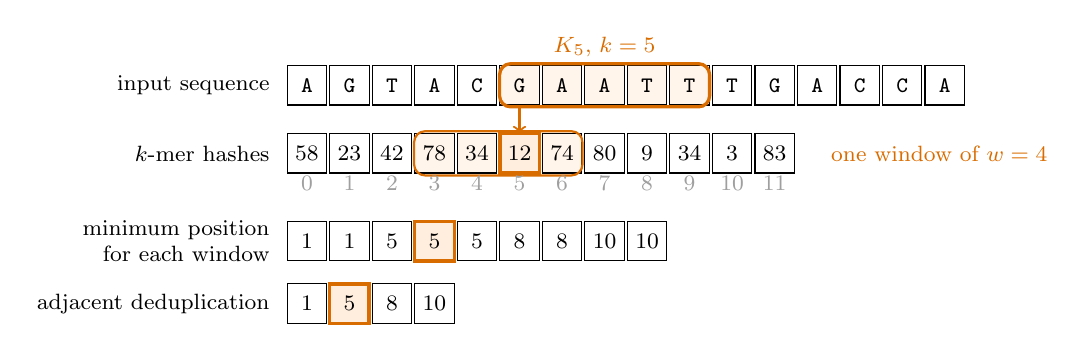
\begin{tikzpicture}[
  x=.54cm,
  y=.72cm,
  font=\footnotesize,
  cell/.style={draw,minimum width=.50cm,minimum height=.50cm,inner sep=0pt},
  tracked/.style={draw=orange!85!black,very thick,fill=orange!13,
                  minimum width=.50cm,minimum height=.50cm,inner sep=0pt},
  context/.style={draw,fill=orange!8,minimum width=.50cm,
                  minimum height=.50cm,inner sep=0pt}
]
  \node[anchor=east] at (4.35,4.10) {input sequence};
  \foreach \i/\v in {0/A,1/G,2/T,3/A,4/C,5/G,6/A,7/A,8/T,9/T,10/T,11/G,12/A,13/C,14/C,15/A}
    \node[cell] (s\i) at (5+\i,4.10) {\texttt{\v}};
  \foreach \i/\v in {5/G,6/A,7/A,8/T,9/T}
    \node[context] at (5+\i,4.10) {\texttt{\v}};
  \draw[orange!85!black,very thick,rounded corners]
    (9.53,3.72) rectangle (14.47,4.48);
  \node[orange!85!black] at (12,4.78) {$K_5$, $k=5$};

  \node[anchor=east] at (4.35,2.90) {$k$-mer hashes};
  \foreach \i/\v in {0/58,1/23,2/42,3/78,4/34,5/12,6/74,7/80,8/9,9/34,10/3,11/83}
    \node[cell] (h\i) at (5+\i,2.90) {\v};
  \foreach \i/\v in {3/78,4/34,6/74}
    \node[context] at (5+\i,2.90) {\v};
  \node[tracked] at (10,2.90) {12};
  \draw[orange!85!black,thick,rounded corners]
    (7.52,2.51) rectangle (11.48,3.29);
  \node[anchor=west,orange!85!black] at (17.10,2.90)
    {one window of $w=4$};
  \foreach \i in {0,...,11}
    \node[gray!75] at (5+\i,2.37) {\i};

  \node[anchor=east,align=right] at (4.35,1.35)
    {minimum position\\for each window};
  \foreach \i/\v in {0/1,1/1,2/5,3/5,4/5,5/8,6/8,7/10,8/10}
    \node[cell] at (5+\i,1.35) {\v};
  \node[tracked] at (8,1.35) {5};

  \node[anchor=east] at (4.35,.25) {adjacent deduplication};
  \foreach \i/\v in {0/1,1/5,2/8,3/10}
    \node[cell] at (5+\i,.25) {\v};
  \node[tracked] at (6,.25) {5};
  \draw[->,thick,orange!85!black] (s5.south) to[out=-90,in=90] (h5.north);
\end{tikzpicture}
\caption{Minimizer extraction for $k=5$ and $w=4$ with illustrative hashes.
Positions in this walkthrough are zero-based $k$-mer starts. BioSeqDB's packed
minimap-compatible record converts them to final-base positions. The
highlighted candidate has hash 12 and remains minimal for three consecutive
windows, so adjacent deduplication emits its position once.}
\label{fig:minimizer-walkthrough}
\end{figure}

Figure~\ref{fig:seed-hash-table} uses fixed four-base seeds on both sides. The
symbols $h_1$, $h_2$, and $h_3$ are some computed hashes.

\begin{figure}[htbp]
\centering
\begin{tikzpicture}[
  x=.88cm,
  y=.82cm,
  font=\footnotesize,
  >=Latex,
  stage/.style={draw,rounded corners,fill=blue!8,align=center,
                minimum height=.72cm},
  seq/.style={draw=orange!75!black,rounded corners,fill=orange!8,
              align=center,minimum height=.72cm},
  index/.style={draw,very thick,rounded corners,fill=yellow!14,
                align=left,inner sep=5pt},
  output/.style={draw=ForestGreen!70!black,rounded corners,
                 fill=green!7,align=left,inner sep=5pt}
]
  \node[font=\small\bfseries] at (3.1,4.55) {Build the reference index};
  \node[seq,minimum width=5.7cm] (ref) at (3.1,3.65)
    {reference: \texttt{GCTATTACCTTAATGTGATGGAC}};
  \node[stage,minimum width=5.7cm] (rseed) at (3.1,2.55)
    {extract $k=4$: \texttt{GCTA}@0, \texttt{TTAA}@9,
     \texttt{ATGT}@12};
  \node[stage,minimum width=5.7cm] (rhash) at (3.1,1.45)
    {hash: $h_1$, $h_2$, $h_3$};

  \node[index] (table) at (5.8,-1.10) {
    \begin{tabular}{@{}cl@{}}
      \textbf{key} & \textbf{occurrence payload} \\
      $h_1$ & $(\textit{ref},0,+)$ \\
      $h_2$ & $(\textit{ref},9,+)$ \\
      $h_3$ & $(\textit{ref},12,+)$
    \end{tabular}};

  \node[font=\small\bfseries] at (11.2,4.55) {Query the index};
  \node[seq,minimum width=5.2cm] (query) at (11.2,3.65)
    {query: \texttt{AGGCTATAACCCTAATGT}};
  \node[stage,minimum width=5.2cm] (qseed) at (11.2,2.55)
    {extract $k=4$: \texttt{GCTA}@2, \texttt{TAAC}@6,
     \texttt{ATGT}@14};
  \node[stage,minimum width=5.2cm] (qhash) at (11.2,1.45)
    {hash and look up: $h_1$, $h_4$, $h_3$};
  \node[output] (anchors) at (11.2,-1.10) {
    \begin{tabular}{@{}l@{}}
      candidate anchors\\
      $(q=2,t=0,+)$\\
      $(q=14,t=12,+)$
    \end{tabular}};

  \draw[->,thick] (ref) -- (rseed);
  \draw[->,thick] (rseed) -- (rhash);
  \draw[->,thick] (rhash) to[out=-90,in=160] (table.west);
  \draw[->,thick] (query) -- (qseed);
  \draw[->,thick] (qseed) -- (qhash);
  \draw[->,thick,blue!65!black] (qhash) to[out=-90,in=30] (table.east);
  \draw[->,thick,ForestGreen!70!black] (table.east) -- (anchors.west);
  \draw[->,thick,red!70!black] (qhash.east) to[out=0,in=90]
    node[pos=.55,right,align=left,text=red!70!black] {$h_4$: absent\\no anchor}
    (13.9,-.10);
\end{tikzpicture}
\caption{Reference-index construction and query lookup. Positions are seed
starts in this example. A usable seed index stores some seed metadata like position and strand}
\label{fig:seed-hash-table}
\end{figure}

Frequent seeds can produce very large occurrence lists. BioSeqDB can exclude
seeds whose target frequency exceeds a configured threshold before anchors
are constructed. This is common practice in other software as well: minimap2 can remove most common minimizers for specific sequence by using percentage threshold ($$\text{--q-occ-frac} \text{[0..1]}$$)

\section{Methods of minimizer generation}

\subsection{Scalar rescan}

The most straightforward algorithm to select smallest hash in a given sliding window is to implement scalar rescan. We keep track of current minimum until it leaves the window. Then we need to do "rescan" part which calculates new minimum from scratch.
Additionally we perform deduplication of adjacent hashes, so if the minimum is unchanged, we don't emit new minimizer. However if there's new equal hash on different position, then we treat that as a new minimizer.

This approach is implemented by minimap2.

\begin{figure}[H]
\centering
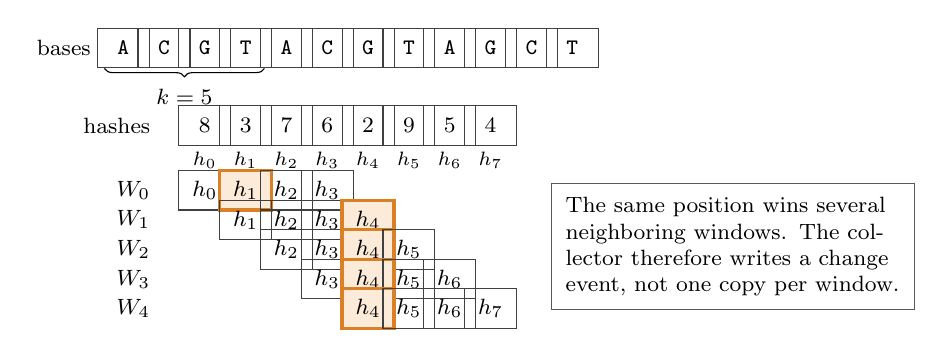
\begin{tikzpicture}[x=.72cm,y=.67cm,font=\footnotesize]
  \foreach \i/\b in {0/A,1/C,2/G,3/T,4/A,5/C,6/G,7/T,8/A,9/G,10/C,11/T}
    \node[rewrite cell,font=\ttfamily\footnotesize] at (.55+\i*.72,4.95) {\b};
  \node[anchor=east] at (.15,4.95) {bases};
  \draw[decorate,decoration={brace,mirror,amplitude=3pt}]
    (.22,4.56)--(3.04,4.56)
    node[midway,below=4pt] {$k=5$};

  \foreach \i/\v in {0/8,1/3,2/7,3/6,4/2,5/9,6/5,7/4}
    \node[rewrite cell] at (1.99+\i*.72,3.48) {\v};
  \node[anchor=east] at (1.20,3.48) {hashes};
  \foreach \i in {0,...,7}
    \node[font=\scriptsize,anchor=north] at (1.99+\i*.72,3.16) {$h_{\i}$};

  \foreach \row/\start/\winner in {0/0/1,1/1/4,2/2/4,3/3/4,4/4/4} {
    \pgfmathsetmacro{\yy}{2.25-.56*\row}
    \node[anchor=east] at (1.20,\yy) {$W_{\row}$};
    \foreach \j in {0,...,3} {
      \pgfmathtruncatemacro{\idx}{\start+\j}
      \pgfmathparse{int(\idx==\winner)}
      \ifnum\pgfmathresult=1
        \node[rewrite min] at (1.99+\idx*.72,\yy) {$h_{\idx}$};
      \else
        \node[rewrite cell] at (1.99+\idx*.72,\yy) {$h_{\idx}$};
      \fi
    }
  }
  \node[rewrite note,text width=4.25cm,anchor=west] at (8.10,1.18)
    {The same position wins several neighboring windows.  The collector
     therefore writes a change event, not one copy per window.};
\end{tikzpicture}
\caption{Minimizer extraction with illustrative $k=5$, $w=4$ hashes.  Each
row is one window of four adjacent $k$-mers. Orange marks the selected
position.  The hash value 2 remains selected while the window moves, so those
windows do not require repeated output.}
\label{fig:rewrite-minimap-walkthrough}
\end{figure}

Equal hashes at different positions are not duplicate records. We wanmt to keep both to guarantee higher minimizer density.

\begin{figure}[H]
\centering
\begin{tikzpicture}[font=\footnotesize]
  \node[anchor=west,font=\bfseries] at (0,4.20)
    {(a) Two positions have the same minimum hash};
  \node[anchor=east] at (1.40,3.52) {$W_0$};
  \foreach \i/\v/\sty in {0/8/rewrite cell,1/3/rewrite min,
                            2/7/rewrite cell,3/3/rewrite min}
    \node[\sty] at (1.90+.74*\i,3.52) {\v};
  \node[anchor=west] at (5.05,3.52)
    {hash 3 occurs at two different positions};

  \node[anchor=west,font=\bfseries] at (0,2.62)
    {(b) The next candidate is larger};
  \node[anchor=east] at (1.40,1.94) {$W_1$};
  \foreach \i/\v/\sty in {0/3/rewrite cell,1/7/rewrite cell,
                            2/3/rewrite min,3/9/rewrite new}
    \node[\sty] at (1.90+.74*\i,1.94) {\v};
  \node[rewrite note,text width=5.0cm,anchor=west] at (5.05,1.94)
    {The rightmost 3 remains the saved minimum.  The earlier 3 is still a
     different identity and can require its own event.};

  \draw[rewrite flow] (3.00,1.42) |- (3.95,.72);
  \node[rewrite out,minimum width=1.55cm] at (4.80,.72) {3 at right};
  \node[rewrite out,minimum width=1.70cm] at (6.65,.72) {tied 3 at left};
\end{tikzpicture}
\caption{Why a hash value alone does not define the output.  Both orange
cells have hash 3, but they refer to different $k$-mer positions.  Minimap2
keeps the rightmost equal position as its saved minimum and has explicit
rules for writing other tied identities.}
\label{fig:rewrite-minimap-ties}
\end{figure}

Minimap2 stores the most recent $w$ candidates in a circular buffer  It also
stores the current minimum and the array slot containing it.

\begin{figure}[H]
\centering
\begin{tikzpicture}[font=\footnotesize]
  \node[anchor=west,font=\bfseries] at (0,4.55) {(a) Cheap step};
  \node at (2.65,4.12) {before};
  \foreach \i/\v/\sty in {0/8/rewrite cell,1/2/rewrite min,
                            2/7/rewrite cell,3/6/rewrite cell}
    \node[\sty] at (1.55+.72*\i,3.48) {\v};
  \draw[rewrite flow] (4.18,3.48)--(4.82,3.48);
  \node[align=center] at (4.50,2.95) {drop 8\quad add 5};
  \node at (6.25,4.12) {after};
  \foreach \i/\v/\sty in {0/2/rewrite min,1/7/rewrite cell,
                            2/6/rewrite cell,3/5/rewrite new}
    \node[\sty] at (5.18+.72*\i,3.48) {\v};
  \node[rewrite note,text width=3.75cm,anchor=west] at (8.35,3.48)
    {2 is still inside the window. Compare only $5>2$: O(1) work};

  \node[anchor=west,font=\bfseries] at (0,2.18) {(b) Expensive step};
  \node at (2.65,1.75) {before};
  \foreach \i/\v/\sty in {0/2/rewrite min,1/7/rewrite cell,
                            2/6/rewrite cell,3/5/rewrite cell}
    \node[\sty] at (1.55+.72*\i,1.10) {\v};
  \draw[rewrite flow] (4.18,1.10)--(4.82,1.10);
  \node[align=center] at (4.50,.58) {drop 2\quad add 9};
  \node at (6.25,1.75) {after};
  \foreach \i/\v in {0/7,1/6,2/5,3/9}
    \node[rewrite new] at (5.18+.72*\i,1.10) {\v};
  \node[rewrite min] at (5.18+.72*2,1.10) {5};
  \draw[draw=rewriteOrange!90!black,very thick]
    (4.80,.72) rectangle (7.72,1.48);
  \node[rewrite note,text width=3.75cm,anchor=west] at (8.35,1.10)
    {2 leaves. Read all $w=4$ live slots and choose 5: $O(w)$.};
\end{tikzpicture}
\caption{The two costs of one minimap2 window advance. Gray cells are already
in the ring, blue is the entering candidate, and orange is the saved or newly
found minimum. A normal step performs one comparison. When the saved minimum
leaves, the algorithm reads the complete window again (rescan)}
\label{fig:rewrite-minimap-rescan}
\end{figure}

Minimap2 stores kmers and apply hash function each time from scratch.

\begin{algorithm}[H]
\caption{Scalar minimap2-style rescan}
\label{alg:rewrite-minimap-rescan}
\small
\begin{enumerate}
  \item Store $k$-mer binary representation and its reverse complement and update them each step. Calculate hash for both of them and take the minimum.
  \item Write this hash into the next slot of the $w$-slot circular buffer.
  \item If new hash is less than or equal to the saved minimum, emit new minimizer.
  \item Else, if the overwritten slot held the current minimum, emit new minimizer and scan all $w$ slots from oldest to newest, and save the
        rightmost record having the smallest hash as new minimum.
  \item At the end of the sequence, write the remaining saved minimum from buffer as final minimizers.
\end{enumerate}
\end{algorithm}

\section{A1: Naive SIMD rescan}
\label{sec:rewrite-naive-simd}

Let's assume we have scalar linear iteration over data. The first though is to unroll the loop so each element of a SIMD vector corresponds to one iteration. This approach however works only if each iteration step is independent.
If we have any condition that requires knowledege of results of previous step the SIMD vector's elements will be dependent on each other and won't give us any advantage. The other approach would be to threat each element not as consecutive input items, but as separate entities handling different parts of the input. Each lane will handle separate parts of iteration, so we will avoid data dependency of vector's elements on each other and replace it with the 
dependency between current state vector and previous state vector.
In this document, I will define a SIMD lane as one numbered element of a vector register.

Each SIMD lane will load fragments of input data:

\begin{figure}[H]
\centering
\begin{tikzpicture}[
  font=\footnotesize,
  context/.style={draw,fill=gray!16,minimum height=.46cm,inner sep=0pt},
  mainspan/.style={draw=blue!70!black,fill=blue!8,
                    minimum height=.46cm,inner sep=0pt},
  cell/.style={draw,minimum width=.62cm,minimum height=.46cm,inner sep=0pt},
  inputcell/.style={draw=blue!70!black,fill=blue!8,
                    minimum width=.62cm,minimum height=.46cm,inner sep=0pt},
  mincell/.style={draw=orange!85!black,very thick,fill=orange!13,
                  minimum width=.62cm,minimum height=.46cm,inner sep=0pt},
  maskcell/.style={draw,fill=gray!10,minimum width=.62cm,
                    minimum height=.42cm,inner sep=0pt},
  outcell/.style={draw=orange!85!black,thick,fill=orange!10,
                  minimum width=1.42cm,minimum height=.48cm,inner sep=2pt},
  stage/.style={draw,minimum width=2.25cm,minimum height=.96cm,
                text width=2.00cm,align=center,inner sep=3pt},
  flow/.style={-{Latex[length=1.8mm]},thick}
]
  \node[anchor=west,font=\bfseries] at (.25,10.65)
    {(a) One SIMD lane per overlapping sequence chunk};

  \foreach \r/\start in {0/1.65,1/3.35,2/5.05,3/6.75} {
    \pgfmathsetmacro{\yy}{9.95-.54*\r}
    \node[anchor=east] at (1.43,\yy) {lane \r};
    \draw[fill=gray!16] (\start,{\yy-.23})
      rectangle ({\start+.78},{\yy+.23});
    \draw[draw=blue!70!black,fill=blue!8] ({\start+.78},{\yy-.23})
      rectangle ({\start+2.48},{\yy+.23});
  }
  \draw[fill=gray!16] (9.72,10.12) rectangle (10.18,10.48);
  \node[anchor=west] at (10.32,10.30) {warm-up context};
  \draw[draw=blue!70!black,fill=blue!8]
    (9.72,9.55) rectangle (10.18,9.91);
  \node[anchor=west] at (10.32,9.73) {later lane steps};
  \node[anchor=north west,align=left,text width=3.05cm] at (9.48,9.30)
    {Chunk starts are separated.  Each read span repeats context from the
      neighbouring region.};
    
  \node[anchor=west,font=\bfseries] at (0,7.08)
    {(b) Lane 0 loses its minimum; the shared branch scans all lanes};
  \foreach \r/\lab in {0/lane 0,1/lane 1,2/lane 2,3/lane 3}
    \node[anchor=east] at (1.35,3.35-.48*\r) {\lab};
  \foreach \r/\c/\v in {
      0/0/7,0/1/6,0/2/5,0/3/9,
      1/0/3,1/1/7,1/2/6,1/3/5,
      2/0/8,2/1/1,2/2/4,2/3/6,
      3/0/5,3/1/6,3/2/2,3/3/8}
    \node[rewrite new] at (1.80+.70*\c,3.35-.48*\r) {\v};
  \node[rewrite min] at (1.80+.70*2,3.35) {5};
  \node[rewrite box,minimum width=2.45cm] (mask) at (6.10,2.63)
    {expiry mask\\$[1,0,0,0]$};
  \draw[rewrite flow] (4.28,2.63)--(mask.west);
  \node[rewrite note,text width=4.0cm,anchor=west] at (7.55,2.63)
    {Only lane 0 accepts a replacement. The processor still loads and
     compares all four vector slots.};
  \draw[draw=rewriteOrange!90!black,very thick]
    (1.43,1.25) rectangle (4.24,3.72);
  \node[rewrite box,fill=rewriteOrange!12,minimum width=4.0cm]
    at (5.95,.62) {$w=4$ vector loads and comparisons};\node[anchor=west,font=\bfseries] at (0,4.08)
    {(b) Lane 0 loses its minimum; the shared branch scans all lanes};
  \foreach \r/\lab in {0/lane 0,1/lane 1,2/lane 2,3/lane 3}
    \node[anchor=east] at (1.35,3.35-.48*\r) {\lab};
  \foreach \r/\c/\v in {
      0/0/7,0/1/6,0/2/5,0/3/9,
      1/0/3,1/1/7,1/2/6,1/3/5,
      2/0/8,2/1/1,2/2/4,2/3/6,
      3/0/5,3/1/6,3/2/2,3/3/8}
    \node[rewrite new] at (1.80+.70*\c,3.35-.48*\r) {\v};
  \node[rewrite min] at (1.80+.70*2,3.35) {5};
  \node[rewrite box,minimum width=2.45cm] (mask) at (6.10,2.63)
    {expiry mask\\$[1,0,0,0]$};
  \draw[rewrite flow] (4.28,2.63)--(mask.west);
  \node[rewrite note,text width=4.0cm,anchor=west] at (7.55,2.63)
    {Only lane 0 accepts a replacement. The processor still loads and
     compares all four vector slots.};
  \draw[draw=rewriteOrange!90!black,very thick]
    (1.43,1.25) rectangle (4.24,3.72);
  \node[rewrite box,fill=rewriteOrange!12,minimum width=4.0cm]
    at (5.95,.62) {$w=4$ vector loads and comparisons};
  
\end{tikzpicture}
\caption{Why direct SIMD rescan is costly. Each lane follows a different
sequence piece. A nonzero expiry mask enters one shared loop over all $w$
vector slots. Masking protects lanes 1--3 from changing their answers, but it
does not remove their loads and comparisons.}
\label{fig:rewrite-naive-simd-rescan}
\end{figure}

Note that algorithm fundamentally stays the same, we only now divided input sequence into chunks and translated each operation (hashing, comparisons) into SIMD instructions:

\begin{algorithm}[H]
\caption{SIMD minimap2-style rescan, with the output cases stated plainly}
\label{alg:simd-minimap-rescan}
\small
\begin{enumerate}
  \item Split input sequence into chunks each corresponding to the lane of SIMD vector. Each lane handles different chunk (chunks overlap slightly to make sure we don't omit any window)
  \item Store $k$-mer binary representations and its reverse complements and update them each step for each lane. Calculate hashes for both of them and take the minimum for each lane.
  \item Write all hashes for each laneinto the next slot of the $w$-slot circular buffer (this buffer now stores SIMD vectors instead of single hashes).
  \item If the new hash vector is less than equal to the minimum vector element-wise, extract corresponding elements and emit new minimizers.
  \item Else (new hash vector is greater then minimum vector on each position), if the overwritten slot held the current minimum for any lane, emit new minimizers and scan all $w$ slots from oldest to newest, and save the
        new minimums vector.
  \item At the end of the sequence, emit all remaining minimums as final minimizers.
\end{enumerate}
\end{algorithm}

As you can see this algorithm works well only if new hash values are greater than current minimum on each position. If not, we still have branching. This is problematic as vectorized algorithms works well if the branching is minimal and CPU pipeline isn't penalized for wrong branch prediction.
Even if we assume the predictor is perfect, we still do expensive rescan for each lane if at least one needs to be updated. Assume one lane needs a rescan with probability $1/w$, then a group of $L$
independent lanes enters the shared slow path with probability
\[
  1-\left(1-\frac1w\right)^L.
\]
For $w=10$ and $L=4$, this is about $34.4\%$. This means that we will need to duplicate work much more often than in scalar case.

\begin{table}[H]
\centering
\small
\begin{tabularx}{\linewidth}{p{.20\linewidth}XX}
\toprule
Method & What happens when one candidate enters & Why it matters here \\
\midrule
Saved minimum plus rescan & Compare once; scan all $w$ slots only when the
saved record leaves & Excellent scalar common case; one expiring SIMD lane
starts shared work \\
Monotone deque & Remove expired records at the front and larger records at the
back & The number of removals depends on the hash values \\
Prefix and suffix minima & Rebuild a fixed block summary every $w$ steps and
combine two saved values per crossing window & The instruction schedule
depends on the step number, not on which lane contains the minimum \\
\bottomrule
\end{tabularx}
\caption{Three ways to maintain a sliding minimum. The next section uses the
third method because every lane performs the same fixed steps.}
\label{tab:rewrite-sliding-minimum-methods}
\end{table}

\section{A2: Two-stack algorithm}
\label{sec:rewrite-sea-simd-minimizers}

In different approach we can preserve prefix and suffix minima to calculate the window minima wrom both of them. SIMD-minimizers paper introduces this approach as well as usage of rolling hashes (nthash) instead of calculating hash each time from scratch. \cite{groot_koerkamp_simd_minimizers_2025}

\subsection{One window minimum from two saved values}

Split the hash stream into blocks of $w$ values.  Within each block, let
$P_i$ be the smallest value from the block start through position $i$, and let
$Q_i$ be the smallest value from position $i$ through the block end.  A window
starting at $j$ and ending at $e=j+w-1$ crosses one block boundary and has
minimum
\[
  \min(Q_j,P_e).
\]
The suffix values are recalculated in a fixed $w$-step loop each $w$ steps. This means that we still have "rescan" part, but it becames unconditional.


\begin{figure}[htbp]
\centering
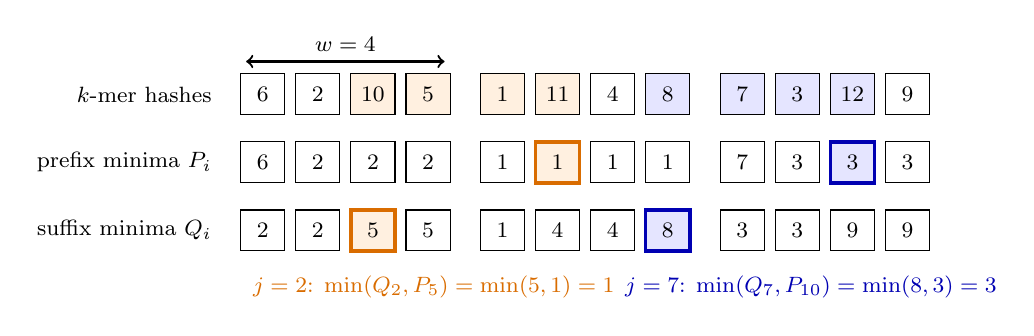
\begin{tikzpicture}[
  x=.70cm,
  y=.72cm,
  font=\footnotesize,
  cell/.style={draw,minimum width=.56cm,minimum height=.52cm,inner sep=0pt},
  first/.style={draw=orange!85!black,very thick,fill=orange!12,
                minimum width=.56cm,minimum height=.52cm,inner sep=0pt},
  second/.style={draw=blue!70!black,very thick,fill=blue!10,
                  minimum width=.56cm,minimum height=.52cm,inner sep=0pt}
]
  \node[anchor=east] at (4.25,3.25) {$k$-mer hashes};
  \foreach \i/\x/\v in {0/5.00/6,1/6.00/2,2/7.00/10,3/8.00/5,
                            4/9.35/1,5/10.35/11,6/11.35/4,7/12.35/8,
                            8/13.70/7,9/14.70/3,10/15.70/12,11/16.70/9}
    \node[cell] (a\i) at (\x,3.25) {\v};
  \foreach \i/\x/\v in {2/7.00/10,3/8.00/5,4/9.35/1,5/10.35/11}
    \node[cell,fill=orange!12] at (\x,3.25) {\v};
  \foreach \i/\x/\v in {7/12.35/8,8/13.70/7,9/14.70/3,10/15.70/12}
    \node[cell,fill=blue!10] at (\x,3.25) {\v};
  \draw[<->,thick] (4.70,3.83) -- (8.30,3.83)
    node[midway,above] {$w=4$};

  \node[anchor=east] at (4.25,2.05) {prefix minima $P_i$};
  \foreach \i/\x/\v in {0/5.00/6,1/6.00/2,2/7.00/2,3/8.00/2,
                            4/9.35/1,5/10.35/1,6/11.35/1,7/12.35/1,
                            8/13.70/7,9/14.70/3,10/15.70/3,11/16.70/3}
    \node[cell] (p\i) at (\x,2.05) {\v};
  \node[first] at (10.35,2.05) {1};
  \node[second] at (15.70,2.05) {3};

  \node[anchor=east] at (4.25,.85) {suffix minima $Q_i$};
  \foreach \i/\x/\v in {0/5.00/2,1/6.00/2,2/7.00/5,3/8.00/5,
                            4/9.35/1,5/10.35/4,6/11.35/4,7/12.35/8,
                            8/13.70/3,9/14.70/3,10/15.70/9,11/16.70/9}
    \node[cell] (q\i) at (\x,.85) {\v};
  \node[first] at (7.00,.85) {5};
  \node[second] at (12.35,.85) {8};

  \node[anchor=west,orange!85!black] at (4.65,-.15)
    {$j=2$: $\min(Q_2,P_5)=\min(5,1)=1$};
  \node[anchor=west,blue!70!black] at (11.40,-.15)
    {$j=7$: $\min(Q_7,P_{10})=\min(8,3)=3$};
\end{tikzpicture}
\caption{Sliding minima from blockwise prefixes and suffixes. Blocks have the
same width as the minimizer window. The two shaded crossing windows each use
one suffix value from the starting block and one prefix value from the ending
block.}
\label{fig:two-stack-minimum}
\end{figure}

The SIMD-Minimizers use fixed-vector size architecture, where the SIMD vector is set to be uint32 times 8. The split per lane is the same as discussed previously. On Neon architecture only 128-bit-wide register is available, so the 256 fixed vector generates separate store intructions.

\begin{figure}[htbp]
\centering
\begin{tikzpicture}[
  x=.64cm,
  y=.68cm,
  font=\footnotesize,
  >=Latex,
  owned/.style={draw=blue!70!black,fill=blue!10,minimum height=.58cm},
  halo/.style={draw=orange!80!black,fill=orange!12,minimum height=.58cm},
  stage/.style={draw,rounded corners,fill=gray!8,align=center,
                minimum width=2.25cm,minimum height=1.05cm,inner sep=3pt}
]
  \node[anchor=east] at (1.30,6.05) {sequence $S$};
  \draw[thick] (1.55,5.72) rectangle (19.65,6.38);
  \foreach \x in {5.55,9.55,13.55,17.55}
    \draw[gray!70] (\x,5.72) -- (\x,6.38);
  \foreach \x/\v in {3.55/$C_0$,7.55/$C_1$,11.55/$C_2$,15.55/$C_3$}
    \node at (\x,6.05) {\v};
  \node at (18.60,6.05) {$\cdots$};

  \draw[owned] (1.55,4.55) rectangle (5.55,5.13);
  \draw[halo] (5.55,4.55) rectangle (7.55,5.13);
  \node at (3.55,4.84) {$C_0$ owned};
  \node at (6.55,4.84) {context};
  \draw[owned] (5.55,3.65) rectangle (9.55,4.23);
  \draw[halo] (9.55,3.65) rectangle (11.55,4.23);
  \node at (7.55,3.94) {$C_1$ owned};
  \node at (10.55,3.94) {context};
  \node[anchor=west] at (12.05,4.38)
    {$g=k+w-2$ bases of context};
  \node[anchor=west,gray!75] at (12.05,3.82)
    {remaining chunks follow the same rule};
  \draw[->] (3.55,5.70) -- (3.55,5.16);
  \draw[->] (7.55,5.70) -- (7.55,4.27);

  \node[stage] (lanes) at (2.15,1.55)
    {lane matrix\\$C_0[t]\quad C_1[t]$\\$C_2[t]\quad C_3[t]$};
  \node[stage] (hash) at (6.25,1.55)
    {rolling hashes\\$h_{0,t}\quad h_{1,t}$\\$h_{2,t}\quad h_{3,t}$};
  \node[stage] (minimum) at (10.35,1.55)
    {window argmin\\$p_{0,t}\quad p_{1,t}$\\$p_{2,t}\quad p_{3,t}$};
  \node[stage] (absolute) at (14.45,1.55)
    {absolute positions\\$p_{c,t}+o_c$};
  \node[stage] (collect) at (18.55,1.55)
    {collected output\\$p_0,p_1,p_2,\ldots$\\deduplicate identity};
  \draw[->,thick] (lanes) -- (hash);
  \draw[->,thick] (hash) -- (minimum);
  \draw[->,thick] (minimum) -- (absolute);
  \draw[->,thick] (absolute) -- (collect);
  \draw[->,thick] (7.55,3.55) to[out=-90,in=90] (lanes.north);
\end{tikzpicture}
\caption{Vectorized minimizer extraction over logical chunks. Each chunk owns
a disjoint range and reads enough context to complete its boundary windows.
Lane-wise rolling hashes and minima produce local positions. Adding each chunk
origin and deduplicating full identities yields a global sketch. The symbolic
chunk size is an execution parameter rather than part of minimizer semantics.}
\label{fig:vector-minimizer-pipeline}
\end{figure}


Note that in this setup we can store full minimum vectors and later use matrix transposition to deduplicate them (in case that minimum stays the same over window):
At first, one SIMD vector contains the selected positions for several
far-apart streams at the same step.  After several steps, the SIMD-Minimizers paper algorithm
rearranges that output matrix so one row contains consecutive windows from
one stream.  Consecutive windows often select the same position.  Once those
positions are adjacent in a row, the paper compares neighbors and keeps only
positions that changed.  Finally, when the ordered stream results are joined,
it removes the repeated boundary position caused by the overlapping input
pieces.


\begin{figure}[htbp]
\centering
\begin{tikzpicture}[
  x=.62cm,
  y=.62cm,
  font=\footnotesize,
  >=Latex,
  cell/.style={draw,minimum width=.52cm,minimum height=.52cm,inner sep=0pt},
  trace/.style={draw=orange!85!black,very thick,fill=orange!12,
                minimum width=.52cm,minimum height=.52cm,inner sep=0pt},
  carry/.style={draw=gray!70,fill=gray!10,text=gray!80,
                minimum width=.52cm,minimum height=.52cm,inner sep=0pt}
]
  \node[font=\small\bfseries] at (2.50,4.15) {events by vector step};
  \foreach \r/\c/\v in {0/0/1,0/1/12,0/2/23,0/3/30,
                            1/0/1,1/1/13,1/2/23,1/3/35,
                            2/0/2,2/1/13,2/2/23,2/3/35,
                            3/0/4,3/1/13,3/2/23,3/3/36}
    \node[cell] at (1+\c,3-\r) {\v};
  \foreach \r/\v in {0/1,1/1,2/2,3/4}
    \node[trace] at (1,3-\r) {\v};

  \node[font=\small\bfseries] at (9.00,4.15) {one sorted row per chunk};
  \foreach \r/\c/\v in {0/0/1,0/1/1,0/2/2,0/3/4,
                            1/0/12,1/1/13,1/2/13,1/3/13,
                            2/0/23,2/1/23,2/2/23,2/3/23,
                            3/0/30,3/1/35,3/2/35,3/3/36}
    \node[cell] at (7.5+\c,3-\r) {\v};
  \foreach \c/\v in {0/1,1/1,2/2,3/4}
    \node[trace] at (7.5+\c,3) {\v};

  \draw[->,very thick] (5.05,1.5) -- (6.75,1.5)
    node[midway,above] {transpose};
  \draw[->,very thick] (11.65,1.5) -- (13.15,1.5)
    node[midway,above,align=center] {deduplicate\\and append};

  \node[font=\small\bfseries] at (16.1,4.15) {ragged chunk outputs};
  \node at (14.2,3.65) {$\operatorname{last}[c]$};
  \foreach \r/\v in {0/0,1/11,2/23,3/30}
    \node[carry] at (14.2,3-\r) {\v};
  \foreach \x/\v in {15.5/1,16.5/2,17.5/4}
    \node[trace] at (\x,3) {\v};
  \foreach \x/\v in {15.5/12,16.5/13}
    \node[cell] at (\x,2) {\v};
  \node[anchor=west,gray!75] at (15.25,1) {no new position};
  \foreach \x/\v in {15.5/35,16.5/36}
    \node[cell] at (\x,0) {\v};
  \foreach \r in {0,...,3}
    \draw[->,gray!70] (14.55,3-\r) -- (15.10,3-\r);
\end{tikzpicture}
\caption{Transposition and boundary deduplication for four logical chunks.
The input rows are vector steps and the columns are chunks. Transposition
makes each chunk a sorted row. Each row has its own previous-position carry,
shown in gray. Only new positions are appended, so padding cells are not part
of the output.}
\label{fig:transpose-dedup}
\end{figure}

\section{A3: Adjacent-window SIMD}
\label{sec:rewrite-v8}

If we want to keep minimap2 hash behaviour the simplest efficient "SIMDification" of scalar approach is as follows:












Past V8 adopted the paper's useful way of finding window minima: each lane
followed a far-apart input piece, every lane kept prefix and suffix summaries,
and the suffix pass ran on a fixed schedule.  The complete algorithm was still
different.  V8 selected with a cheaper key derived from the canonical packed
$k$-mer, deferred the full minimap-style scramble until output, resolved an
equal key with its packed local position, and appended selected lanes through
a scalar loop.  It did not implement the paper's output transpose and
cross-stream join removal.  Its ring and summaries were fixed arrays; no
\texttt{std::map} was part of the minimum calculation.

The inspected V8 snapshot also contains two representation errors, separate
from the intended algorithm.  For the usual 32-bit, $k=15$ form, the mask used
for the multiplied ordering key retains only fourteen useful hash bits.  In a
64-bit instantiation of the same expression, its two masks do not overlap and
the ordering hash becomes zero.  The code also stores strand in the low bit of
the packed canonical word and clears that bit before calculating the emitted
minimap-style hash.  A word whose original low bit was one therefore receives
the wrong emitted hash.  These errors are additional reasons not to treat V8
output as an exact minimap2 stream; they are not properties of the
prefix/suffix method itself.

\begin{figure}[H]
\centering
\begin{tikzpicture}[font=\footnotesize]
  \node[anchor=west,font=\bfseries] at (0,8.10)
    {(a) One V8 lane follows one far-apart, overlapping input piece};
  \foreach \r/\x in {0/.65,1/2.25,2/3.85,3/5.45} {
    \pgfmathsetmacro{\yy}{7.38-.52*\r}
    \node[anchor=east] at (.48,\yy) {lane \r};
    \draw[fill=rewriteGray!20] (\x,\yy-.22) rectangle (\x+.72,\yy+.22);
    \draw[fill=rewriteBlue!14,draw=rewriteBlue!90!black]
      (\x+.72,\yy-.22) rectangle (\x+2.32,\yy+.22);
  }
  \node[rewrite note,text width=4.30cm,anchor=west] at (8.05,6.62)
    {Neighboring lanes read some of the same bases. Their minimum state does
     not cross the lane boundary.};

  \node[anchor=west,font=\bfseries] at (0,5.12)
    {(b) SIMD calculates four independent window minima};
  \foreach \r/\lab in {0/L0,1/L1,2/L2,3/L3}
    \node[anchor=east] at (1.05,4.43-.48*\r) {\lab};
  \foreach \r/\c/\v in {
      0/0/9,0/1/4,0/2/7,0/3/2,
      1/0/8,1/1/3,1/2/6,1/3/5,
      2/0/6,2/1/1,2/2/8,2/3/4,
      3/0/7,3/1/5,3/2/2,3/3/6}
    \node[rewrite cell] at (1.48+.67*\c,4.43-.48*\r) {\v};
  \foreach \r/\c/\v in {0/3/2,1/1/3,2/1/1,3/2/2}
    \node[rewrite min] at (1.48+.67*\c,4.43-.48*\r) {\v};
  \node[rewrite box,minimum width=2.35cm,text width=1.95cm] (fixed)
    at (5.60,3.72) {fixed prefix/suffix combine};
  \draw[rewrite flow] (4.02,3.72)--(fixed.west);
  \foreach \r/\v in {0/2,1/3,2/1,3/2}
    \node[rewrite min] at (7.34,4.43-.48*\r) {\v};
  \node[rewrite note,text width=4.15cm,anchor=west] at (7.95,3.72)
    {The minimum update is vectorized. The branch is controlled by the shared
     step counter, not by a lane's hash.};

  \node[anchor=west,font=\bfseries] at (0,2.02)
    {(c) Sparse output returns to scalar lane handling};
  \node[rewrite box,minimum width=2.30cm,text width=1.95cm] (store)
    at (2.00,.74) {store hash, position, strand, and mask};
  \node[rewrite box,minimum width=2.25cm,text width=1.90cm] (loop)
    at (5.00,.74) {scalar loop over lane 0 to lane 3};
  \node[rewrite out,minimum width=1.65cm] at (8.00,1.09) {lane 1 record};
  \node[rewrite out,minimum width=1.65cm] at (8.00,.37) {lane 3 record};
  \draw[rewrite flow] (store)--(loop);
  \draw[rewrite flow] (loop.east)-|(7.05,1.09);
  \draw[rewrite flow] (loop.east)-|(7.05,.37);
  \node[rewrite note,text width=3.6cm,anchor=west] at (9.10,.74)
    {Only repetition within one lane is suppressed. Overlap records from two
     neighboring lanes can remain.};
\end{tikzpicture}
\caption{Past V8 lane processing. Input lanes are far apart, the
prefix/suffix minimum is calculated with SIMD operations, and sparse records
are appended by a scalar lane loop. V8 has an input rearrangement for distant
pieces, but it has no SIMD-Minimizers output rearrangement and join removal.}
\label{fig:rewrite-v8-lanes}
\end{figure}

\begin{table}[H]
\centering
\footnotesize
\begin{tabularx}{\linewidth}{p{.18\linewidth}XX}
\toprule
Question & SIMD-Minimizers & Past V8 \\
\midrule
What is one lane? & One of eight far-apart, overlapping input streams & One
far-apart, overlapping input piece \\
How is the hash advanced? & Rolling forward and reverse ntHash & Rolling
canonical packed word with a cheaper multiplied ordering key; full
minimap-style mix delayed until output \\
How is the minimum found? & Block prefixes and suffixes & The same
prefix/suffix minimum structure \\
How is an equal minimum chosen? & For an odd complete span, more G/T than A/C
selects the leftmost occurrence; otherwise the rightmost occurrence is
selected & Packed local position selects one earlier equal key;
complete minimap2 tie events are not reproduced \\
How is output collected? & Rearrange vector-step output into stream rows and
remove repeated join identities & Store vectors, inspect lanes in scalar code,
and suppress repetition only within a lane \\
Is a tree map used? & No & No \\
\bottomrule
\end{tabularx}
\caption{The shared prefix/suffix minimum does not make V8 and SIMD-Minimizers the
same complete algorithm. Their hash, equal-minimum rule, and output handling
differ.}
\label{tab:rewrite-sea-v8-differences}
\end{table}

\section{Current BioSeq algorithms and the route selected by the benchmark}
\label{sec:rewrite-current-bioseq}

The public name
\begin{center}
\footnotesize
\texttt{bioseq\_block\_simd\_dp\_}\\
\texttt{two\_stack\_nthash\_no\_index}
\end{center}
preserves names from earlier development.  Static routing is more specific:
the named large no-index case maps target pieces and the query through the
state-carrying adjacent-window SIMD routine.  Its active window-minimum loop
does not call the separate whole-input prefix/suffix routine and does not call
the bounded rolling-ntHash routine.  The phrase \emph{adjacent-window
routine} is used below because lane~0 handles one window, lane~1 handles the
very next window, and so on.

\begin{figure}[H]
\centering
\begin{tikzpicture}[font=\footnotesize]
  \node[rewrite box,minimum width=7.25cm,fill=rewriteGray!15] (name)
    at (6.30,6.35)
    {named E2E row:\\
     \texttt{bioseq\_block\_simd\_dp\_}\\
     \texttt{two\_stack\_nthash\_no\_index}};
  \node[rewrite box,minimum width=4.20cm] (select) at (6.30,5.05)
    {public selector \texttt{TWO\_STACK\_NTHASH}\\chooses the exact SIMD family};
  \draw[rewrite flow] (name)--(select);

  \node[rewrite box,minimum width=4.25cm,fill=rewriteBlue!12] (target)
    at (3.20,3.45) {each target segment\\state carried to the next segment};
  \node[rewrite box,minimum width=4.25cm,fill=rewriteBlue!12] (query)
    at (9.40,3.45) {query sketch\\same exact seed rules};
  \draw[rewrite flow] (select.south) |- (target.north);
  \draw[rewrite flow] (select.south) |- (query.north);

  \node[rewrite box,minimum width=5.15cm,fill=rewriteOrange!14] (adj)
    at (6.30,1.90) {adjacent-window SIMD block\\exact minimap-style hash and ties};
  \draw[rewrite flow] (target.south) |- (adj.west);
  \draw[rewrite flow] (query.south) |- (adj.east);

  \node[rewrite note,text width=4.45cm,anchor=west,fill=rewriteGray!10]
    at (.35,.35) {Not selected here: whole-input \texttt{vector\_stream}
    two-stack control.};
  \node[rewrite note,text width=4.45cm,anchor=west,fill=rewriteGray!10]
    at (7.85,.35) {Not selected here: bounded rolling-ntHash scheme.};
\end{tikzpicture}
\caption{What the named no-index E2E row actually runs. Both target segments
and the query use the state-carrying adjacent-window SIMD routine. The
words ``two stack'' and ``nthash'' in the public row name do not describe the
active inner minimum or hash in this route.}
\label{fig:rewrite-current-e2e-route}
\end{figure}

\subsection{The adjacent-window calculation}

Let $B$ be the number of candidate positions handled together.  The routine
retains the last $k-1$ bases and the last $w-1$ candidate records.  It adds $B$
new consecutive bases, forms $B$ consecutive $k$-mers, calculates the exact
minimap-style hash for each, and places the retained and new candidates next
to one another.  It then makes $w$ shifted SIMD loads.  Lane $j$ is the whole
window beginning at the $j$th candidate, so lanes are neighboring windows in
this routine.  This is the opposite of V8, where lanes are far-apart input
pieces.

\begin{figure}[H]
\centering
\begin{tikzpicture}[font=\footnotesize]
  \node[anchor=west,font=\bfseries] at (0,9.05)
    {(a) Retained context plus $B$ new consecutive positions};
  \node[rewrite box,minimum width=4.0cm,fill=rewriteGray!18] (basesold)
    at (2.35,8.28) {last $k-1$ bases};
  \node[rewrite box,minimum width=2.40cm,fill=rewriteBlue!14] (basesnew)
    at (5.75,8.28) {$B$ new bases};
  \node[rewrite box,minimum width=4.05cm] (make) at (9.65,8.28)
    {$B$ consecutive canonical $k$-mers\\and exact minimap-style hashes};
  \draw[rewrite flow] (basesold.east)--(basesnew.west);
  \draw[rewrite flow] (basesnew.east)--(make.west);

  \node[anchor=west,font=\bfseries] at (0,7.28)
    {(b) Four neighboring windows are calculated together ($B=4,w=4$ shown)};
  \node[anchor=east] at (1.78,6.58) {candidate row};
  \foreach \i/\v/\sty in {0/7/rewrite old,1/6/rewrite old,2/5/rewrite old,
                            3/9/rewrite new,4/4/rewrite new,5/8/rewrite new,
                            6/3/rewrite new}
    \node[\sty] at (2.20+.70*\i,6.58) {\v};

  \foreach \r/\lab in {0/$W_0$,1/$W_1$,2/$W_2$,3/$W_3$}
    \node[anchor=east] at (1.78,5.82-.54*\r) {\lab};
  \foreach \r/\c/\v in {
      0/0/7,0/1/6,0/2/5,0/3/9,
      1/0/6,1/1/5,1/2/9,1/3/4,
      2/0/5,2/1/9,2/2/4,2/3/8,
      3/0/9,3/1/4,3/2/8,3/3/3}
    \node[rewrite cell] at (2.20+.70*\c,5.82-.54*\r) {\v};
  \foreach \r/\c/\v in {0/2/5,1/3/4,2/2/4,3/3/3}
    \node[rewrite min] at (2.20+.70*\c,5.82-.54*\r) {\v};

  \node[rewrite box,minimum width=2.45cm] (reduce) at (6.38,5.02)
    {$w$ shifted loads\\and $\leq$ reduction};
  \draw[rewrite flow] (5.02,5.02)--(reduce.west);
  \foreach \r/\v in {0/5,1/4,2/4,3/3}
    \node[rewrite min] at (8.32,5.82-.54*\r) {\v};
  \node[rewrite note,text width=3.80cm,anchor=west] at (8.92,5.02)
    {One lane is one complete window. The next lane is the window one
     candidate position to the right.};

  \node[anchor=west,font=\bfseries] at (0,3.15)
    {(c) The ordinary output path writes only changed selections};
  \node[anchor=east] at (1.93,2.45) {previous};
  \node[anchor=east] at (1.93,1.88) {current};
  \node[anchor=east] at (1.93,1.31) {write?};
  \foreach \i/\v in {0/5@3,1/5@3,2/4@5,3/4@5}
    \node[rewrite old,minimum width=.93cm] at (2.48+.98*\i,2.45) {\v};
  \foreach \i/\v in {0/5@3,1/4@5,2/4@5,3/3@7}
    \node[rewrite new,minimum width=.93cm] at (2.48+.98*\i,1.88) {\v};
  \foreach \i/\v in {0/0,1/1,2/0,3/1}
    \node[rewrite cell,minimum width=.93cm] at (2.48+.98*\i,1.31) {\v};
  \node[rewrite box,minimum width=2.35cm,fill=rewriteGreen!13] (compress)
    at (7.45,1.88) {compressed store\\of marked lanes};
  \draw[rewrite flow] (5.95,1.88)--(compress.west);
  \node[rewrite out,minimum width=1.28cm] at (9.55,2.20) {5@3};
  \node[rewrite out,minimum width=1.28cm] at (9.55,1.55) {4@5};
  \node[rewrite note,text width=2.55cm,anchor=west] at (10.35,1.88)
    {3@7 remains saved until a later event.};
\end{tikzpicture}
\caption{The current adjacent-window minimum with small values for
legibility. Gray candidates come from the preceding block and blue candidates
are new. Four lanes hold four neighboring windows. The real $k=15,w=10$
specialization reads ten shifted vectors and produces $B$ window minima.}
\label{fig:rewrite-current-adjacent-windows}
\end{figure}

The comparison uses $\leq$, so a later equal-hash position replaces an earlier
one.  Ordinary changes form one lane mask and are written in a compressed
batch.  Equal hashes at several different positions can require several
records for one window.  That rare case rearranges an event matrix so all
records for $W_0$ precede all records for $W_1$, and so on.  The rearrangement
restores output order; it is not a deduplication pass.

\begin{figure}[H]
\centering
\begin{tikzpicture}[font=\footnotesize]
  \node[font=\bfseries] at (2.45,5.32) {before: one row per event slot};
  \foreach \c/\lab in {0/$W_0$,1/$W_1$,2/$W_2$,3/$W_3$}
    \node at (1.35+.78*\c,4.72) {\lab};
  \foreach \r/\lab in {0/old,1/tie 1,2/tie 2}
    \node[anchor=east] at (.87,4.12-.56*\r) {\lab};
  \foreach \r/\c/\v in {0/0/a,0/1/b,0/2/--,0/3/f,
                          1/0/c,1/1/--,1/2/e,1/3/g,
                          2/0/d,2/1/--,2/2/--,2/3/--}
    \node[rewrite cell] at (1.35+.78*\c,4.12-.56*\r) {\v};

  \node[rewrite box,minimum width=1.85cm] (swap) at (5.60,3.55)
    {rows become\\columns};
  \draw[rewrite flow] (4.28,3.55)--(swap.west);
  \draw[rewrite flow] (swap.east)--(6.83,3.55);

  \node[font=\bfseries] at (9.18,5.32) {after: one row per window};
  \foreach \c/\lab in {0/old,1/tie 1,2/tie 2}
    \node at (8.05+.90*\c,4.72) {\lab};
  \foreach \r/\lab in {0/$W_0$,1/$W_1$,2/$W_2$,3/$W_3$}
    \node[anchor=east] at (7.53,4.12-.56*\r) {\lab};
  \foreach \r/\c/\v in {0/0/a,0/1/c,0/2/d,
                          1/0/b,1/1/--,1/2/--,
                          2/0/--,2/1/e,2/2/--,
                          3/0/f,3/1/g,3/2/--}
    \node[rewrite cell] at (8.05+.90*\c,4.12-.56*\r) {\v};

  \node[rewrite out,minimum width=2.25cm] at (2.10,.85) {a\quad c\quad d};
  \node[rewrite out,minimum width=.85cm] at (3.82,.85) {b};
  \node[rewrite out,minimum width=.85cm] at (4.78,.85) {e};
  \node[rewrite out,minimum width=1.55cm] at (6.02,.85) {f\quad g};
  \node[rewrite note,text width=5.25cm,anchor=west] at (7.05,.85)
    {Every named record remains. Only empty sentinel cells disappear.};
\end{tikzpicture}
\caption{Rare equal-minimum output in the current adjacent-window routine.
The matrix is rearranged to put records in window order. A compressed store
removes empty cells; it does not compare or remove two real records.}
\label{fig:rewrite-current-event-order}
\end{figure}

\subsection{State across input fragments}

A normal storage-fragment boundary does not end the biological sequence.  The
routine retains at most $k-1$ bases, fewer than one incomplete vector group,
$w-1$ candidates, and the selected record of the last complete window.  An
ambiguous base is different: it clears the valid $k$-mer run and advances a
maximum-valued candidate through the window.

\begin{figure}[H]
\centering
\begin{tikzpicture}[font=\footnotesize]
  \draw[fill=rewriteGray!18] (.55,4.55) rectangle (5.35,5.25);
  \node at (2.95,4.90) {packed fragment $f_i$};
  \draw[fill=rewriteBlue!14,draw=rewriteBlue!90!black]
    (7.05,4.55) rectangle (11.85,5.25);
  \node at (9.45,4.90) {packed fragment $f_{i+1}$};
  \draw[rewrite flow] (5.35,4.90)--(7.05,4.90);
  \node[above,align=center] at (6.20,5.05) {storage boundary\\no reset};

  \node[rewrite box,minimum width=11.30cm,fill=rewriteGray!12] (state)
    at (6.20,3.02) {retained state: $k-1$ bases \quad $w-1$ candidates
      \quad incomplete group \quad selected record};
  \draw[rewrite flow] (4.25,4.50)|-(state.north);
  \draw[rewrite flow] (state.north)-|(8.15,4.50);

  \node[rewrite box,minimum width=9.90cm,fill=rewriteOrange!13] (amb)
    at (6.20,1.40) {ambiguous base: clear the valid $k$-mer context and
      insert a maximum-valued candidate};
  \draw[rewrite flow] (state)--(amb);
  \node[rewrite note,text width=10.8cm,anchor=west] at (.80,.20)
    {Only end-of-input performs the final saved-record write. A fragment
     boundary and an ambiguous base therefore have different effects.};
\end{tikzpicture}
\caption{Bounded continuation in the current adjacent-window SIMD path. State is carried
across a normal storage boundary, so a window can cross it without rereading
an overlapping chunk. An ambiguous base resets the valid $k$-mer run but does
not masquerade as end-of-input.}
\label{fig:rewrite-current-continuation}
\end{figure}

\begin{algorithm}[H]
\caption{Current $k=15,w=10$ adjacent-window block, simplified}
\label{alg:rewrite-current-adjacent-block}
\small
\begin{enumerate}
  \item Join retained base context with $B$ new positions and build $B$
        consecutive forward and reverse-complement $k$-mers.
  \item Choose each canonical $k$-mer, mark invalid or palindromic candidates
        with a maximum sentinel, and calculate the exact minimap-style hash.
  \item Join the retained $w-1$ candidate tail with the $B$ new candidates.
        Read $w$ shifted vectors and reduce with $\leq$; lane $j$ now contains
        the minimum of the $j$th neighboring window.
  \item Form masks for a smaller entering value, an expired saved record,
        first-window output, and final output.
  \item On the common path, compressed-store the marked records.  If equal
        hashes at different identities are present, build the tie-event
        matrix, rearrange it into window order, and compressed-store all real
        cells.
  \item Retain the final base context, candidate tail, incomplete group, and
        selected record for the next input fragment.
\end{enumerate}
\end{algorithm}

\subsection{Why this complete route can be faster than V8}

The current minimum operation is not an asymptotically cheaper form of V8's
two-stack minimum.  V8 rebuilds $w$ suffix entries once every $w$ steps.  The
current routine makes $w$ shifted comparisons for every group of $B$ adjacent
windows and also calculates the exact selection hash.  A speed advantage, when
measured, must therefore come from the complete route around that reduction:

\begin{itemize}
  \item new $k$-mers come from one short consecutive input region, rather than
        from an input rearrangement of far-apart pieces;
  \item state crosses ordinary fragments directly, without overlapping lane
        reads and their repeated join records;
  \item the ordinary output is written as one compressed batch rather than by
        visiting every lane in scalar code; and
  \item the larger exact tie calculation runs only after a hash precheck says
        it is needed.
\end{itemize}

Those are code-level reasons, not timing results.  Section
\ref{sec:rewrite-performance-evidence} keeps the older measurements separate
and does not present them as a V8-versus-current measurement.

\subsection{Other current minimizer routes}

BioSeq has several routes because they do not all produce the same seed
stream. In particular, the three values assigned to
\texttt{dispatch.params.minimizer\_algorithm} select three different ways of
making minimizers. They do not select the prefilter, chaining method, or final
alignment method; those are chosen by other fields. The same minimizer setting
is used for the query and target so that a query seed can be found in the
target table.

\subsubsection{What the three ordinary benchmark settings mean}

The ordinary alignment benchmark normally supplies DNA4 packed into 32-bit
words, with the complete query and target already available in memory, and
uses $k=15,w=10$. Under those conditions the three assignments in the
benchmark source mean the following.

\begin{description}
  \item[\texttt{two\_stack\_nthash}.]
    The four \texttt{bioseq\_prefilter\_*} rows and the six ordinary alignment
    rows whose names contain \texttt{two\_stack\_nthash} run the whole-input
    descendant of V8. One lane follows one far-apart part of the sequence. It
    advances packed forward and reverse-complement $k$-mers, updates a prefix
    minimum, and rebuilds suffix minima once every $w$ positions. Long inputs
    advance two independent Highway vector groups. Despite the setting's
    historical name, this route does not calculate ntHash. The E2E caller
    shown earlier uses the same setting but supplies the target as pieces and
    requires exact minimap-style output for its target table, so it
    deliberately selects the adjacent-window algorithm instead.

  \item[\texttt{bounded\_nthash\_simd}.]
    The two ordinary rows whose names contain \texttt{bounded\_nthash} call
    the bounded-input entry point. The query is processed as one range and the
    target as one or more ranges. Every range uses eight logical ntHash
    streams and the prefix/suffix minimum. This is the maintained successor of
    the old \texttt{PAPER\_NTHASH\_SIMD} setting. It is the BioSeq algorithm
    closest to SIMD-Minimizers, but its exact hash and tied-minimum output differ from
    the paper, as explained below.

  \item[\texttt{simd\_minimap2\_reference}.]
    This setting is used by the ordinary slow-reference row. It runs the naive
    SIMD rescan from
    Figure~\ref{fig:rewrite-naive-simd-rescan}. One lane follows one far-apart
    sequence part and saves one minimum. If any lane loses its saved minimum,
    the shared loop reads all $w$ vector slots; masks ensure that only expired
    lanes change their answer.
\end{description}

Words such as \texttt{ksw2}, \texttt{block}, \texttt{prefilter}, or
\texttt{vulkan\_tiled\_dp} elsewhere in an ordinary row name describe later
mapping work. They do not change the minimizer route just described. Highway
chooses the available processor target and physical lane count; there is no
separate handwritten AVX algorithm. If a required input shape is unsupported,
the checked SIMD setting reports failure. It does not silently change to the
scalar minimizer after entering that checked route.

\subsubsection{The whole-input prefix/suffix route}

When \texttt{two\_stack\_nthash} receives one complete, already available
DNA4 sequence stored in 32-bit words with $k=15,w=10$, it can choose the
whole-input descendant of V8.  This is the route reached by the ordinary
in-memory benchmark names that contain \texttt{two\_stack\_nthash}.  Each lane
owns a far-apart sequence piece.  The code shifts packed forward and
reverse-complement words, ranks their canonical word with the multiplied
ordering key, updates a prefix minimum, and rebuilds suffix minima every $w$
steps.  Long inputs advance two independent Highway lane groups together.

This route still does not calculate ntHash.  It applies the minimap-style mix
only when it emits, stores SIMD results to arrays, and then visits output lanes
with scalar code.  It has no state format for continuing through ordinary
input fragments.  For these reasons it cannot be substituted for the
adjacent-window route while a target index and query are being built from
pieces.

\begin{table}[H]
\centering
\footnotesize
\begin{tabularx}{\linewidth}{p{.22\linewidth}p{.22\linewidth}X
  p{.10\linewidth}}
\toprule
Minimizer setting & Input for this row & Actual algorithm & Named
no-index E2E? \\
\midrule
\texttt{scalar} & DNA4 or DNA5 scalar input & saved minimum plus occasional
ring rescan & no \\
\shortstack[l]{\texttt{simd\_minimap2\_}\\\texttt{reference}} &
one complete DNA4 input & distant
lane streams with one saved minimum per lane and a shared SIMD rescan & no \\
\texttt{two\_stack\_nthash} & a target table or input supplied in pieces &
neighboring windows, full $w$-slot SIMD reduction, minimap-style hash & yes \\
\texttt{two\_stack\_nthash} & complete DNA4 stored in 32-bit words,
$k=15,w=10$ &
distant lane streams with V8-descended prefix/suffix minima & no \\
\texttt{bounded\_nthash\_simd} & DNA4 query or bounded target range,
$k=15,w=10$ & eight rolling-ntHash streams with prefix/suffix minima & no \\
\shortstack[l]{\texttt{vulkan\_minimap\_}\\\texttt{integer}} &
supported GPU and input & many GPU
tiles, each using a serial minimap-style ring/rescan & no \\
\bottomrule
\end{tabularx}
\caption{Current minimizer settings and their actual inner algorithms.  The
\texttt{two\_stack\_nthash} selector is the confusing case: its caller and
input shape choose between two different algorithms.}
\label{tab:rewrite-current-routing}
\end{table}

\begin{table}[H]
\centering
\footnotesize
\begin{tabularx}{\linewidth}{p{.40\linewidth}XX}
\toprule
Configured run name or family & Query minimizers & Target minimizers \\
\midrule
\shortstack[l]{Named E2E \texttt{two\_stack\_nthash\_}\\
\texttt{no\_index}} & adjacent-window SIMD &
adjacent-window SIMD while building a temporary target table \\
\shortstack[l]{Named E2E \texttt{two\_stack\_nthash\_}\\
\texttt{just\_index}} & adjacent-window SIMD &
matching adjacent-window target index built before mapping \\
Ordinary \texttt{bioseq\_prefilter\_*} and names containing
\texttt{two\_stack\_nthash} & whole-input V8 descendant & whole-input V8
descendant \\
Ordinary \texttt{simd\_minimap2\_slow} & direct SIMD rescan & direct SIMD
rescan \\
Ordinary names containing \texttt{bounded\_nthash} & bounded rolling ntHash &
bounded rolling ntHash \\
Scalar BioSeq rows & scalar rescan & scalar rescan \\
Vulkan-minimizer rows & Vulkan tile rescan & Vulkan tile rescan or its
device target-index builder \\
External minimap2 rows & bundled minimap2 sketch & bundled minimap2 sketch or
its prebuilt index \\
\bottomrule
\end{tabularx}
\caption{What the configured test families actually execute.  This mapping
comes from the current call paths, not from interpreting a historical word in
the displayed run name.  No current configured run calls the old V8 source
body directly.}
\label{tab:rewrite-configured-routes}
\end{table}

\begin{table}[H]
\centering
\footnotesize
\begin{tabularx}{\linewidth}{p{.19\linewidth}XX}
\toprule
Question & Past V8 & Current adjacent-window E2E path \\
\midrule
What is one lane? & One far-apart, overlapping input piece & One of the next
$B$ neighboring windows \\
How is input prepared? & Rearrange packed input so every lane receives the
next base of its own piece & Read consecutive bases and retain $k-1$ bases
across input pieces \\
How is the minimum found? & Update a prefix; rebuild suffixes once per $w$
steps; compare one prefix and suffix & Read $w$ shifted vectors and reduce
each of $B$ complete windows \\
Which hash selects it? & Cheaper multiplied ordering key; full minimap-style
mix delayed until output & Exact minimap-style hash before selection \\
How are normal records written? & Store vectors and inspect lanes in scalar
code & One event mask and one compressed SIMD store \\
What is rearranged? & Input values for far-apart pieces & Rare equal-minimum
output records, solely to restore window order \\
Is there a deduplication pass? & No; suppression is within one lane & No;
unchanged selections are suppressed before output and real ties remain \\
\bottomrule
\end{tabularx}
\caption{Past V8 and the current route selected by the named no-index E2E
row. The current code did not replace V8 with a cheaper two-stack minimum; it
changed lane meaning, input handling, exactness, and record writing.}
\label{tab:rewrite-v8-current}
\end{table}

\subsubsection{How BioSeq bounded ntHash differs from SIMD-Minimizers}

Earlier versions called this route \texttt{PAPER\_NTHASH\_SIMD}, and some
development text abbreviated its output format as PNT1.  It was not removed.
The production route was renamed \texttt{bounded\_nthash\_simd}; its numeric
selector stayed unchanged. Target tables made by this algorithm still carry
the four-letter marker PNT1, which tells the reader that the bounded hash and
tied-position rules were used. The current bounded kernel is therefore the
maintained successor of that earlier production kernel. A different
experimental helper that accepted an unpacked array of base numbers was
removed, but the query, index, and benchmark routes never called that helper.
Restoring the old production source would create a second copy of an
algorithm that is already present.

Here \emph{bounded} means that one call receives a finite DNA range and clear
limits saying which window starts belong to that range. The kernel rereads
enough neighboring bases to rebuild its state; it does not carry rolling-hash
or prefix/suffix state from one storage fragment to the next.

The algorithm always has eight logical input pieces. A Highway target with
eight physical 32-bit lanes holds them in one vector group; a target with four
physical lanes holds them in two groups. The checked implementation rejects
other physical lane counts instead of changing the algorithm.

The current bounded algorithm works as follows.

\begin{enumerate}
  \item It divides one DNA4 range into eight far-apart pieces. Each piece is
        assigned its own interval of window starts; these intervals do not
        overlap. To finish windows at a boundary, a piece needs $k+w-2$ bases
        to its right. Packed reads are rounded to whole 32-bit words and can
        therefore include more bases.
  \item It rearranges packed input words so the next SIMD value contains the
        next DNA letter from every far-apart piece. This is the same kind of
        \emph{input} rearrangement used by SIMD-Minimizers. It removes no output.
  \item Every lane maintains a forward and reverse-complement rolling hash.
        The two unsigned 32-bit values are added, with overflow wrapping back
        into 32 bits, to obtain the value compared inside a window.
  \item Every lane updates a prefix minimum on each step and rebuilds $w$
        suffix minima once per $w$ candidates. One prefix/suffix comparison
        gives the next window minimum. This is the paper's two-stack idea.
  \item If the minimum hash occurs once, the algorithm writes that occurrence.
        If it occurs several times, it writes the leftmost and rightmost
        occurrences; it does not write equal occurrences between them.
  \item While one piece is processed, a record is skipped when its hash,
        position, and forward/reverse mark are identical to the
        preceding selected event for that piece. The first record of each
        later piece is held back and compared with the last record of the
        preceding non-empty piece. An identical boundary record is written
        once.
\end{enumerate}

Step 6 is important: bounded ntHash does \emph{not} implement the paper's
output-matrix rearrangement. SIMD-Minimizers first produces one selected position for
every window, rearranges a block of those positions into one ordered row per
input piece, and then compares neighboring positions in SIMD. Bounded ntHash
instead compares an event with the preceding event while each lane advances,
stores the lane results in small arrays, and appends them with a scalar loop.
Both methods avoid many repeated outputs from neighboring windows, but they do
so at different times and with different instructions.

The hash and tied-minimum rules also differ. These are not small storage
details: they can select different positions from the same DNA sequence.

\begin{table}[H]
\centering
\footnotesize
\begin{tabularx}{\linewidth}{p{.18\linewidth}XX}
\toprule
Question & SIMD-Minimizers & BioSeq bounded ntHash \\
\midrule
How is the rolling value updated? & Use one-bit rotations and a fixed lookup
table. The packed DNA order is A, C, T, G. & Use seven-bit rotations and
BioSeq's own four lookup values. BioSeq's packed DNA order is A, C, G, T. The
resulting 32-bit numbers are therefore not the same as the paper's numbers. \\
How much of the hash chooses the minimum? & Compare only the upper 16 bits;
the lower 16 bits of the packed value hold a local position. & Compare all 32
hash bits and keep the position separately. Two values tied by the paper's
upper 16 bits may be ordered differently here. \\
What happens when the minimum occurs twice? & For odd $k+w-1$, count G/T
against A/C over the complete span. More G/T chooses the leftmost minimum;
otherwise choose the rightmost. Return one occurrence. & Return both extreme
occurrences: leftmost first and rightmost second. \\
How is a forward/reverse value recorded? & The whole-span count chooses an
endpoint; the paper does not attach a per-$k$-mer strand bit to that returned
position. & Mark an endpoint as reverse only when its reverse rolling value
is smaller than its forward value. Equality is marked forward. \\
How are repeated positions removed? & Rearrange an output matrix into one row
per input piece, compare neighboring positions, compact the changes, and
remove the repeated position at a piece join. & Compare with the preceding
record during each lane's walk and compare the last/first records at a piece
join. There is no output-matrix rearrangement. \\
\bottomrule
\end{tabularx}
\caption{A direct comparison of SIMD-Minimizers and BioSeq bounded ntHash. They share
far-apart input pieces, an input rearrangement, rolling forward/reverse hash
state, and prefix/suffix minima. They calculate different hash numbers, make
different choices for tied minima, and remove repeated output by different
methods.}
\label{tab:rewrite-sea-bounded-nthash}
\end{table}

For BioSeq's usual $k=15,w=10$, the complete span has
$k+w-1=24$ bases, which is even. This does not prevent rolling ntHash or the
prefix/suffix minimum, but it does not satisfy the odd-span condition of the
paper's canonical endpoint rule. BioSeq bounded ntHash does not use that
rule; it reports both extreme occurrences of a tied minimum.

\begin{figure}[H]
\centering
\begin{tikzpicture}[font=\footnotesize]
  \node[anchor=west,font=\bfseries] at (0,7.85)
    {(a) One window has the same minimum at two positions};
  \node[anchor=east] at (2.15,6.25) {position};
  \node[anchor=east,align=right] at (2.15,5.58) {compared\\key};
  \foreach \i in {0,...,3}
    \node[rewrite cell] at (2.65+.78*\i,6.25) {\i};
  \foreach \i/\v in {0/9,1/2,2/5,3/2}
    \node[rewrite cell] at (2.65+.78*\i,5.58) {\v};
  \node[rewrite min] at (2.65+.78*1,5.58) {2};
  \node[rewrite min] at (2.65+.78*3,5.58) {2};

  \node[rewrite box,text width=3.30cm,minimum width=3.65cm,
        fill=rewriteBlue!10] at (7.25,6.12)
    {SIMD-Minimizers, odd span:\\more G/T selects position 1; otherwise
     position 3; write one};
  \node[rewrite box,text width=3.30cm,minimum width=3.65cm,
        fill=rewriteOrange!12] at (11.15,6.12)
    {BioSeq bounded:\\write positions 1 and 3; mark each reverse only if its
     reverse hash is smaller};

  \node[anchor=west,font=\bfseries] at (0,4.35)
    {(b) Repeated selections from neighboring windows};
  \node[rewrite box,minimum width=2.25cm] (events) at (1.70,3.05)
    {positions\\$[1,1,5,5]$};
  \node[rewrite box,text width=3.70cm,minimum width=4.05cm,
        fill=rewriteBlue!10] (seaout) at (5.40,3.05)
    {SIMD-Minimizers:\\rearrange output into one row per input piece; compare
     neighboring positions};
  \node[rewrite out,minimum width=1.85cm] (searesult) at (8.70,3.05)
    {$[1,5]$};
  \draw[rewrite flow] (events)--(seaout);
  \draw[rewrite flow] (seaout)--(searesult);

  \node[rewrite box,minimum width=2.25cm] (eventsb) at (1.70,1.05)
    {positions\\$[1,1,5,5]$};
  \node[rewrite box,text width=3.70cm,minimum width=4.05cm,
        fill=rewriteOrange!10] (boundout) at (5.40,1.05)
    {bounded:\\compare each event with the preceding event while its input
     piece is being processed};
  \node[rewrite out,minimum width=1.85cm] (boundresult) at (8.70,1.05)
    {$[1,5]$};
  \draw[rewrite flow] (eventsb)--(boundout);
  \draw[rewrite flow] (boundout)--(boundresult);
  \node[rewrite note,text width=3.05cm,anchor=west] at (9.85,2.05)
    {At an input-piece join, bounded ntHash also compares the preceding
     piece's last record with the next piece's first record.};
\end{tikzpicture}
\caption{Two visible output differences. The small numbers in panel (a) are
the keys seen by the minimum comparison: the paper obtains them from the
upper 16 hash bits, while bounded ntHash normally compares all 32 bits.
SIMD-Minimizers
returns one end of this tie, while bounded ntHash returns both ends. Panel (b)
shows that the same simple run of repeated positions can reduce to the same
two outputs, but SIMD-Minimizers first rearranges an output matrix whereas bounded ntHash
compares successive events during the lane walk.}
\label{fig:rewrite-sea-bounded-output}
\end{figure}

Because these choices can produce different hashes and different positions,
the bounded query must be compared with a target table made by the bounded
algorithm. The named \texttt{two\_stack\_nthash} E2E rows do not select it.
The ordinary rows whose names contain \texttt{bounded\_nthash} do.

\subsubsection{Vulkan: many serial tile walks run together}

On the GPU, a segment is a memory-sized part of a large input, not one
minimizer window.  A segment includes context around an owned core.  Inside
the uploaded segment, each shader invocation owns a smaller tile.  It starts
before the tile, replays enough bases to rebuild rolling and window state, and
then writes only events triggered inside its half-open owned interval.  The
window minimum inside one tile is the same saved-minimum plus ring-rescan
method shown in Figure~\ref{fig:rewrite-minimap-rescan}; it is not a
prefix/suffix minimum.

Because the number of output events is not known in advance, the compact
route runs a count pass, an exclusive scan of tile counts, and an emit pass.
Each tile receives a non-overlapping output range before it writes.

\begin{figure}[H]
\centering
\begin{tikzpicture}[font=\footnotesize]
  \node[anchor=west,font=\bfseries] at (0,10.45)
    {(a) One memory segment has context around its owned core};
  \draw[fill=rewriteGray!20] (.55,9.50) rectangle (2.55,10.18);
  \draw[fill=rewriteBlue!14,draw=rewriteBlue!90!black]
    (2.55,9.50) rectangle (10.55,10.18);
  \draw[fill=rewriteGray!20] (10.55,9.50) rectangle (12.55,10.18);
  \node at (1.55,9.84) {context};
  \node at (6.55,9.84) {owned core};
  \node at (11.55,9.84) {context};

  \node[anchor=west,font=\bfseries] at (0,8.88)
    {(b) Tile invocations own adjacent trigger intervals};
  \draw[fill=rewriteGray!20] (.55,7.90) rectangle (2.40,8.58);
  \draw[fill=rewriteBlue!14,draw=rewriteBlue!90!black]
    (2.40,7.90) rectangle (6.15,8.58);
  \draw[fill=rewriteGray!20] (4.30,6.80) rectangle (6.15,7.48);
  \draw[fill=rewriteBlue!14,draw=rewriteBlue!90!black]
    (6.15,6.80) rectangle (9.90,7.48);
  \node at (1.48,8.24) {replay};
  \node at (4.28,8.24) {tile $i$ owns $[b_i,e_i)$};
  \node at (5.23,7.14) {replay};
  \node at (8.03,7.14) {tile $i+1$ owns next interval};
  \draw[densely dashed,rewriteGray!90] (6.15,6.48)--(6.15,8.85);
  \node[anchor=west] at (10.20,7.69)
    {$e_i=b_{i+1}$};

  \node[anchor=west,font=\bfseries] at (0,5.98)
    {(c) One tile walks positions in order and uses a ring with rescan};
  \node at (.65,4.98) {$\cdots$};
  \foreach \i/\v/\sty in {0/2/rewrite min,1/7/rewrite old,2/6/rewrite old,
                            3/5/rewrite new,4/9/rewrite cell,5/4/rewrite cell,
                            6/3/rewrite cell}
    \node[\sty] at (1.25+.72*\i,4.98) {\v};
  \draw[very thick,rewriteGray!90] (3.06,4.55)--(3.06,5.41);
  \draw[draw=rewriteOrange!90!black,very thick]
    (.88,4.50) rectangle (3.82,5.46);
  \node[rewrite note,text width=5.15cm,anchor=west] at (7.05,4.55)
    {Roll one canonical $k$-mer, push it into the $w$-slot ring, compare it
     with the saved minimum, and rescan only when that saved slot leaves.};
  \node[anchor=west,rewriteGray!90!black] at (1.10,4.15)
    {events during replay are not written};

  \node[anchor=west,font=\bfseries] at (0,3.35)
    {(d) Compact output allocation};
  \node[rewrite box,minimum width=2.35cm] (count) at (1.65,2.45)
    {count events\\per tile};
  \node[rewrite box,minimum width=2.35cm] (scan) at (4.72,2.45)
    {exclusive scan\\of counts};
  \node[rewrite box,minimum width=2.35cm] (emit) at (7.79,2.45)
    {replay tile and\\write events};
  \node[rewrite box,minimum width=2.65cm,fill=rewriteGreen!14] (ranges)
    at (11.05,2.45) {separate output\\range for each tile};
  \draw[rewrite flow] (count)--(scan);
  \draw[rewrite flow] (scan)--(emit);
  \draw[rewrite flow] (emit)--(ranges);
  \node[rewrite note,text width=11.3cm,anchor=west] at (.65,.78)
    {Parallelism comes from many tile invocations. Positions inside one tile
     are processed in order because the rolling $k$-mer and saved minimum
     depend on earlier positions.};
\end{tikzpicture}
\caption{How the current Vulkan sketch divides work. Context is read again,
but only the owned core or tile can publish an event. Each tile uses a serial
ring/rescan state machine. Count--scan--emit gives tiles exact, separate
output ranges while many tiles execute at the same time.}
\label{fig:rewrite-vulkan-sketch}
\end{figure}

\subsubsection{Why target and query must use the same minimizer rules}

A target table is looked up by the hash written by its minimizer algorithm.
BioSeq bounded ntHash and the minimap-style algorithms can write different
hashes and different tied positions for the same DNA. If the target table was
made by bounded ntHash but the query was made by adjacent-window SIMD, many
query hashes would simply not exist in that table even when the DNA matched.

BioSeq therefore first asks which minimizer rules made the target table. It
then chooses an implementation that produces exactly those rules. If that
implementation cannot handle the alphabet, $k$, $w$, input layout, or
available Highway lane count, the operation reports an error. Secretly
switching to another minimizer algorithm would produce a plausible-looking
but incorrect lookup.

\begin{figure}[H]
\centering
\begin{tikzpicture}[font=\footnotesize]
  \node[rewrite box,minimum width=3.20cm,fill=rewriteBlue!12] (scheme)
    at (6.20,6.75) {How was the target table made?};
  \node[rewrite box,minimum width=3.10cm] (pntproof) at (2.70,5.00)
    {Can bounded ntHash\\handle this input?};
  \node[rewrite box,minimum width=3.30cm] (mmproof) at (9.70,5.00)
    {Which minimap-style\\implementation was requested?};
  \coordinate (routefork) at (6.20,5.90);
  \draw[thick] (scheme.south)--(routefork);
  \draw[rewrite flow] (routefork)-|(pntproof.north)
    node[pos=.38,above] {bounded ntHash};
  \draw[rewrite flow] (routefork)-|(mmproof.north)
    node[pos=.38,above] {minimap-style};

  \node[rewrite box,minimum width=2.75cm,fill=rewriteGreen!14] (pnt)
    at (2.70,3.45) {bounded ntHash\\SIMD};
  \node[rewrite box,minimum width=2.75cm,fill=rewriteOrange!14] (rejectp)
    at (2.70,1.90) {reject mismatch};
  \draw[rewrite flow] (pntproof)--(pnt) node[midway,right] {yes};
  \draw[rewrite flow] (pntproof.west)-|(rejectp.west)
    node[pos=.25,left] {no};

  \node[rewrite box,minimum width=2.35cm,fill=rewriteGreen!14] (exact)
    at (7.10,3.45) {adjacent-window\\SIMD};
  \node[rewrite box,minimum width=2.35cm,fill=rewriteGreen!14] (vk)
    at (9.70,3.45) {Vulkan};
  \node[rewrite box,minimum width=2.35cm,fill=rewriteGreen!14] (scalar)
    at (12.30,3.45) {Scalar};
  \draw[rewrite flow] (mmproof.south)-|(exact.north);
  \draw[rewrite flow] (mmproof)--(vk);
  \draw[rewrite flow] (mmproof.south)-|(scalar.north);

  \node[rewrite box,minimum width=5.25cm,fill=rewriteOrange!14] (fail)
    at (9.70,1.55) {requested implementation cannot handle input: error};
  \draw[rewrite flow] (exact.south)--++(0,-.45)
    -| ($(fail.north)+(-1.65,0)$);
  \draw[rewrite flow] (vk)--(fail);
  \draw[rewrite flow] (scalar.south)--++(0,-.45)
    -| ($(fail.north)+(1.65,0)$);
\end{tikzpicture}
\caption{Why a checked implementation cannot silently change minimizer
algorithms. The query must use the same hash and tied-position rules as the
target table. Bounded ntHash therefore cannot fall through to a minimap-style
implementation, and a failed adjacent-window or Vulkan check is reported.}
\label{fig:rewrite-backend-selection}
\end{figure}

\section{Performance evidence}
\label{sec:rewrite-performance-evidence}

Timing claims are grouped here so they cannot be mistaken for algorithm
definitions.  The first four charts preserve an older three-run measurement
series.  They are useful history, but they predate the current adjacent-window
route and use a different binary and experiment scope.  Their source retained
means but not the raw samples or sample standard deviations; the figures
therefore show no error bars.  They must not be used as a direct measured
V8-versus-current comparison.

\subsection{Older end-to-end series}

\begin{figure}[H]
  \centering
\begin{CacheMeCode}{python, custom include command={\input{\robExtAddCachePathAndName{\robExtFinalHash.pgf}}}, set placeholder eval={__LINEWIDTH__}{\lenToCmNoUnit[in]{\linewidth}}}
    import matplotlib
    matplotlib.use("pgf")
    import matplotlib.pyplot as plt
    import numpy as np
    matplotlib.rcParams.update({
      "font.family": "serif",
      "font.serif": [],
      "text.usetex": True,
    })
    fig, ax = plt.subplots()
    fig.set_size_inches(__LINEWIDTH__, 0.55*__LINEWIDTH__, forward=True)
    buckets = ['47 kbp', '49 kbp', '52 kbp', '903 kbp', '5.0 Mbp']
    minimap2 = [20.11, 20.10, 20.13, 190.95, 1060.13]
    scalar = [14.56, 14.94, 15.09, 188.93, 1171.0]
    simd_v6 = [15.21, 15.90, 16.05, 201.68, 1207.99]
    v8 = [14.64, 15.07, 15.24, 183.77, 1131.87]
    historical_v13 = [13.78, 14.02, 13.82, 172.38, 1113.3]
    x = np.arange(len(buckets))
    width = 0.16
    ax.bar(x-2*width, minimap2, width, label='minimap2', color='#6F6F6F')
    ax.bar(x-width, scalar, width, label='scalar', color='#B8B8B8')
    ax.bar(x, simd_v6, width, label='naive SIMD rescan', color='#4C78A8')
    ax.bar(x+width, v8, width, label='past V8', color='#F28E2B')
    ax.bar(x+2*width, historical_v13, width,
           label='historical V12/V13 route', color='#59A14F')
    ax.set_xticks(x)
    ax.set_xticklabels(buckets)
    ax.set_yscale('log')
    ax.set_ylabel('wall time per pair (ms, log scale)', fontsize=8)
    ax.tick_params(axis='both', labelsize=7)
    ax.legend(fontsize=7, frameon=False, loc='upper left', ncol=2)
    ax.grid(True, alpha=0.25, axis='y', which='both')
    print(get_filename_from_extension('.pgf'))
    plt.savefig(get_filename_from_extension('.pgf'), bbox_inches='tight')
\end{CacheMeCode}
  \caption{Older end-to-end wall times across five sequence lengths. Each bar
  is the recorded mean of three runs; raw samples and sample standard
  deviations were not retained with this chart. ``Historical V12/V13 route''
  is not the current adjacent-window E2E route. The log scale allows the short
  and long inputs to share one axis.}
  \label{fig:rewrite-historical-headline}
\end{figure}

\subsection{How the older minimizer phase changed}

\begin{figure}[H]
  \centering
\begin{CacheMeCode}{python, custom include command={\input{\robExtAddCachePathAndName{\robExtFinalHash.pgf}}}, set placeholder eval={__LINEWIDTH__}{\lenToCmNoUnit[in]{\linewidth}}}
    import matplotlib
    matplotlib.use("pgf")
    import matplotlib.pyplot as plt
    import numpy as np
    matplotlib.rcParams.update({
      "font.family": "serif",
      "font.serif": [],
      "text.usetex": True,
    })
    fig, ax = plt.subplots()
    fig.set_size_inches(__LINEWIDTH__, 0.53*__LINEWIDTH__, forward=True)
    names = ['V6\nrescan', 'V8\nprefix/suffix', 'V8.5\ndelayed mix',
             'V11\ntwo streams', 'V12\ninlined', 'scalar']
    inner = [23.88, 19.90, 13.60, 13.60, 9.23, 0.0]
    wrapper = [14.94, 12.43, 8.62, 8.62, 5.76, 12.50]
    x = np.arange(len(names))
    ax.bar(x, wrapper, label='recorded wrapper field', color='#4C78A8')
    ax.bar(x, inner, bottom=wrapper, label='recorded inner field',
           color='#F28E2B')
    ax.axhline(12.50, linestyle='--', linewidth=1, color='#6F6F6F',
               label='scalar recorded field')
    for i, total in enumerate(np.array(inner)+np.array(wrapper)):
        ax.text(i, total+0.5, f'{total:.1f}', ha='center', fontsize=7)
    ax.set_xticks(x)
    ax.set_xticklabels(names)
    ax.set_ylabel('recorded time per 903-kbp pair (ms)', fontsize=8)
    ax.tick_params(axis='both', labelsize=7)
    ax.legend(fontsize=7, frameon=False, loc='upper right')
    ax.grid(True, alpha=0.25, axis='y')
    print(get_filename_from_extension('.pgf'))
    plt.savefig(get_filename_from_extension('.pgf'), bbox_inches='tight')
\end{CacheMeCode}
  \caption{Older minimizer-phase fields for one 903-kbp case, recorded as
  means of three runs without retained raw samples or sample standard
  deviations. The chart preserves the original stacked presentation. Before
  using the stack as an additive time, the instrumentation must confirm that
  the wrapper and inner fields are exclusive rather than nested.}
  \label{fig:rewrite-historical-phase-evolution}
\end{figure}

\subsection{Older complete-run phase composition}

\begin{figure}[H]
  \centering
\begin{CacheMeCode}{python, custom include command={\input{\robExtAddCachePathAndName{\robExtFinalHash.pgf}}}, set placeholder eval={__LINEWIDTH__}{\lenToCmNoUnit[in]{\linewidth}}}
    import matplotlib
    matplotlib.use("pgf")
    import matplotlib.pyplot as plt
    import numpy as np
    matplotlib.rcParams.update({
      "font.family": "serif",
      "font.serif": [],
      "text.usetex": True,
    })
    fig, ax = plt.subplots()
    fig.set_size_inches(__LINEWIDTH__, 0.58*__LINEWIDTH__, forward=True)
    configs = ['scalar', 'V6 rescan', 'V8', 'V12 before V13',
               'V12 after V13']
    phases = [
      ('sketch fields', [12.50,38.82,32.43,14.99,14.52], '#4C78A8',''),
      ('target index', [16.0,14.3,14.6,26.38,23.83], '#A0A0A0',''),
      ('seed hits', [6.5,11.0,11.3,12.32,12.0], '#59A14F',''),
      ('chain', [16.0,8.9,8.9,8.88,8.78], '#F28E2B',''),
      ('error estimate', [0.7,7.2,7.1,7.88,0.85], '#F28E2B','//'),
      ('alignment', [87.5,86.4,86.5,87.25,85.42], '#6F6F6F','..'),
    ]
    bottom = np.zeros(len(configs))
    for label, values, color, hatch in phases:
        ax.bar(configs, values, bottom=bottom, label=label, color=color,
               hatch=hatch, edgecolor='#404040', linewidth=.25)
        bottom += np.array(values)
    ax.set_ylabel('recorded time per 903-kbp pair (ms)', fontsize=8)
    ax.tick_params(axis='both', labelsize=7)
    ax.legend(fontsize=6.5, frameon=False, loc='upper right', ncol=2)
    ax.grid(True, alpha=0.25, axis='y')
    plt.xticks(rotation=13, ha='right')
    print(get_filename_from_extension('.pgf'))
    plt.savefig(get_filename_from_extension('.pgf'), bbox_inches='tight')
\end{CacheMeCode}
  \caption{Older phase composition for one 903-kbp experiment. Values are
  recorded means of three runs; no sample standard deviations are available.
  The chart separates a minimizer-side change from the later error-estimation
  change, but it does not describe the current named no-index route.}
  \label{fig:rewrite-historical-phase-stack}
\end{figure}

\subsection{Older percentage view of the same end-to-end series}

\begin{figure}[H]
  \centering
\begin{CacheMeCode}{python, custom include command={\input{\robExtAddCachePathAndName{\robExtFinalHash.pgf}}}, set placeholder eval={__LINEWIDTH__}{\lenToCmNoUnit[in]{\linewidth}}}
    import matplotlib
    matplotlib.use("pgf")
    import matplotlib.pyplot as plt
    import numpy as np
    matplotlib.rcParams.update({
      "font.family": "serif",
      "font.serif": [],
      "text.usetex": True,
    })
    fig, ax = plt.subplots()
    fig.set_size_inches(__LINEWIDTH__, 0.50*__LINEWIDTH__, forward=True)
    buckets = ['47 kbp', '49 kbp', '52 kbp', '903 kbp', '5.0 Mbp']
    scalar = np.array([14.56,14.94,15.09,188.93,1171.0])
    v6 = np.array([15.21,15.90,16.05,201.68,1207.99])
    v8 = np.array([14.64,15.07,15.24,183.77,1131.87])
    old13 = np.array([13.78,14.02,13.82,172.38,1113.3])
    x = np.arange(len(buckets))
    width = .27
    ax.bar(x-width, (v6-scalar)/scalar*100, width,
           label='naive SIMD rescan', color='#4C78A8')
    ax.bar(x, (v8-scalar)/scalar*100, width,
           label='past V8', color='#F28E2B')
    ax.bar(x+width, (old13-scalar)/scalar*100, width,
           label='historical V12/V13 route', color='#59A14F')
    ax.axhline(0, linewidth=.7, color='#6F6F6F')
    ax.axhline(-10, linestyle='--', linewidth=1, color='#A0A0A0',
               label='historical -10\% target')
    ax.set_xticks(x)
    ax.set_xticklabels(buckets)
    ax.set_ylabel('difference from scalar (\%, negative is faster)', fontsize=8)
    ax.tick_params(axis='both', labelsize=7)
    ax.legend(fontsize=7, frameon=False, loc='upper right', ncol=2)
    ax.grid(True, alpha=0.25, axis='y')
    print(get_filename_from_extension('.pgf'))
    plt.savefig(get_filename_from_extension('.pgf'), bbox_inches='tight')
\end{CacheMeCode}
  \caption{Percentage form of the older three-run end-to-end means. This is a
  transformation of Figure~\ref{fig:rewrite-historical-headline}, not an
  independent experiment. Raw samples and sample standard deviations were not
  retained with the chart.}
  \label{fig:rewrite-historical-speedup}
\end{figure}

\subsection{A later historical CPU checkpoint}

A later experiment recorded four complete observations per configuration and
reported their median.  Its bounded-ntHash row used a target index built with
that scheme, while the minimap2 and adjacent-window rows used their matching
seed schemes.  It is therefore
a comparison of complete valid configurations, not interchangeable function
bodies.

\begin{figure}[H]
\centering
\begin{tikzpicture}[x=.82cm,y=.80cm,font=\footnotesize]
  \draw[rewrite flow] (0,0)--(10.9,0) node[right] {sketch time (s)};
  \foreach \x in {0,2,4,6,8,10} {
    \draw (\x,-.08)--(\x,.08);
    \node[below] at (\x,-.08) {\x};
  }
  \fill[rewriteGreen!75] (0,.48) rectangle (2.923,1.10);
  \node[anchor=east] at (-.20,.79) {bounded ntHash};
  \node[anchor=west] at (3.05,.79) {2.923};
  \fill[rewriteGray!75] (0,1.50) rectangle (4.733,2.12);
  \node[anchor=east] at (-.20,1.81) {minimap2};
  \node[anchor=west] at (4.86,1.81) {4.733};
  \fill[rewriteBlue!75] (0,2.52) rectangle (9.256,3.14);
  \node[anchor=east] at (-.20,2.83) {adjacent SIMD};
  \node[anchor=west] at (9.39,2.83) {9.256};
\end{tikzpicture}
\caption{Sketch component in a later historical CPU checkpoint. Each value is
the median of four observations. The retained summary does not provide a
sample standard deviation. Bounded ntHash uses a different target/query seed scheme, so
the chart compares complete configurations rather than identical output.}
\label{fig:rewrite-historical-cpu-checkpoint}
\end{figure}

\subsection{GPU before and after the rolling, all-tiles rewrite}

\begin{table}[H]
\centering
\small
\begin{tabular}{lrrr}
\toprule
GPU sketch version & per-call sketch & throughput & complete probe \\
\midrule
rebuild-heavy, too few active lanes & 272.0\,ms & 73\,Mbp/s & 21.83\,s \\
rolling update, all-tile schedule & 40.3\,ms & 494\,Mbp/s & 11.70\,s \\
\bottomrule
\end{tabular}
\caption{One controlled GPU before/after measurement. The two rows use the
same recorded workload and exact DNA4 output check. Repetition count and
sample spread were not retained in the source summary, so these values should
not be given error bars.}
\label{tab:rewrite-gpu-progression}
\end{table}

\subsection{Limit of the retained measurements}

None of the preserved charts runs past V8 and the current adjacent-window
kernel with the same input, output rule, binary, and timed boundary.  The
figures therefore do not establish a numerical speedup between those two
algorithms.  The supported conclusion is the code-level explanation in
Section~\ref{sec:rewrite-current-bioseq}: the current route removes V8's
far-apart input preparation and scalar lane-output loop, but its window
minimum itself performs more comparisons.

\subsection{Related seed designs retained as visual reference}

The following two figures are retained because they explain terms used when
comparing sketching work, although they are not steps of the E2E minimizer
route described above.  A spaced seed masks positions in one span.  A linked
seed chooses separated components.  BLEND constructs a fuzzy fingerprint by
letting token hashes vote on each output bit.

\begin{figure}[H]
\centering
\begin{tikzpicture}[font=\footnotesize]
  \node[anchor=west,font=\bfseries] at (0,8.85) {(a) Minimizer};
  \foreach \i/\txt/\rank/\sty in {
      0/GCTATTA/161/rewrite cell,1/CTATTAC/2/rewrite min,
      2/TATTACC/252/rewrite cell,3/ATTACCT/69/rewrite cell}
    \node[\sty,minimum width=2.25cm,minimum height=.82cm,align=center]
      at (1.35+2.55*\i,8.02) {\texttt{\txt}\\rank \rank};
  \node[rewrite box,minimum width=2.50cm] (mselect) at (6.45,6.72)
    {choose the\\lowest rank};
  \node[rewrite out,minimum width=2.50cm] (mout) at (10.15,6.72)
    {\texttt{CTATTAC}};
  \foreach \x in {1.35,3.90,6.45,9.00}
    \draw[rewrite flow] (\x,7.58)|-(mselect.north);
  \draw[rewrite flow] (mselect)--(mout);

  \node[anchor=west,font=\bfseries] at (0,5.72) {(b) Spaced seed};
  \node[rewrite box,minimum width=2.25cm] (sin) at (1.50,4.82)
    {\texttt{GCTATTA}\\\texttt{GATACTA}};
  \node[rewrite box,minimum width=2.55cm,fill=rewriteBlue!12] (mask)
    at (4.65,4.82) {mask \texttt{1011011}\\keep the 1 positions};
  \node[rewrite out,minimum width=2.25cm,align=center] (skeep)
    at (7.80,4.82)
    {\texttt{GTATA}\\\texttt{GTATA}};
  \node[rewrite box,minimum width=2.15cm] (shash) at (10.65,4.82)
    {hash retained\\symbols};
  \draw[rewrite flow] (sin)--(mask);
  \draw[rewrite flow] (mask)--(skeep);
  \draw[rewrite flow] (skeep)--(shash);

  \node[anchor=west,font=\bfseries] at (0,3.55) {(c) Linked seed};
  \node[rewrite out,minimum width=1.65cm,align=center] (l1) at (1.30,2.52)
    {$s_1$\\\texttt{GCTA}};
  \node[rewrite box,minimum width=2.25cm] (lw2) at (3.72,2.52)
    {$W_2$ candidates\\\texttt{CCTT}, \texttt{TTAA}};
  \node[rewrite out,minimum width=1.65cm,align=center] (l2) at (6.08,2.52)
    {choose\\\texttt{TTAA}};
  \node[rewrite box,minimum width=2.25cm] (lw3) at (8.45,2.52)
    {$W_3$ candidates\\\texttt{GTGA}, \texttt{TGGA}};
  \node[rewrite out,minimum width=1.65cm,align=center] (l3) at (10.80,2.52)
    {choose\\\texttt{TGGA}};
  \draw[rewrite flow] (l1)--(lw2);
  \draw[rewrite flow] (lw2)--(l2);
  \draw[rewrite flow] (l2)--(lw3);
  \draw[rewrite flow] (lw3)--(l3);
  \node[rewrite note,text width=10.9cm,anchor=west] at (.55,.72)
    {A linked key contains the chosen components. Bases between its component
     windows are not part of the key.};
\end{tikzpicture}
\caption{Three distinct seed constructions. A minimizer selects one complete
$k$-mer by rank. A spaced seed hashes only positions marked by a binary mask.
A linked seed chooses components from explicit downstream windows and joins
those components into one key.}
\label{fig:rewrite-related-seeds}
\end{figure}

\begin{figure}[H]
\centering
\begin{tikzpicture}[font=\footnotesize]
  \node[anchor=west,font=\bfseries] at (0,6.75)
    {(a) BLEND-I on two nearby contiguous seeds};
  \node[rewrite box,minimum width=2.20cm] (b1) at (1.45,5.66)
    {\texttt{GCTATTAC}\\\texttt{GCTACTAC}};
  \node[rewrite box,minimum width=2.50cm,fill=rewriteBlue!12] (tokens)
    at (4.55,5.66) {overlapping\\tokens};
  \node[rewrite box,minimum width=2.40cm] (bits) at (7.52,5.66)
    {ordinary token\\hash bits};
  \node[rewrite box,minimum width=2.15cm,fill=rewriteOrange!14] (vote)
    at (10.28,5.66) {signed vote\\for each bit};
  \node[rewrite out,minimum width=2.05cm,align=center] (fp) at (12.82,5.66)
    {fuzzy\\fingerprint};
  \draw[rewrite flow] (b1)--(tokens);
  \draw[rewrite flow] (tokens)--(bits);
  \draw[rewrite flow] (bits)--(vote);
  \draw[rewrite flow] (vote)--(fp);
  \node[rewrite note,text width=11.9cm,anchor=west] at (.55,4.12)
    {Similar seeds share many token hashes, so many bit votes remain the same.
     A shared fingerprint is possible, not guaranteed.};

  \node[anchor=west,font=\bfseries] at (0,3.25)
    {(b) BLEND-S on linked components};
  \node[rewrite box,minimum width=2.75cm] (linked) at (1.75,2.15)
    {\texttt{GCTA|TTAA|TGGA}};
  \node[rewrite box,minimum width=2.35cm,fill=rewriteBlue!12] (ctok)
    at (5.00,2.15) {component\\token hashes};
  \node[rewrite box,minimum width=2.20cm,fill=rewriteOrange!14] (cvote)
    at (7.90,2.15) {bit vote};
  \node[rewrite box,minimum width=2.20cm] (lookup) at (10.70,2.15)
    {index lookup};
  \node[rewrite out,minimum width=2.10cm,align=center] (verify)
    at (13.35,2.15)
    {candidates\\to verify};
  \draw[rewrite flow] (linked)--(ctok);
  \draw[rewrite flow] (ctok)--(cvote);
  \draw[rewrite flow] (cvote)--(lookup);
  \draw[rewrite flow] (lookup)--(verify);
  \node[rewrite note,text width=11.9cm,anchor=west] at (.55,.57)
    {A fuzzy-key match proposes candidates. It does not establish that the
     underlying sequence regions are equal.};
\end{tikzpicture}
\caption{Fuzzy fingerprint construction in BLEND~\cite{blend}. Token hashes
vote independently on each output bit. Nearby seeds can retain enough votes
to share a fingerprint, after which downstream work still verifies the
candidate match.}
\label{fig:rewrite-blend-fuzzy-hash}
\end{figure}

\section*{Chapter conclusion}

Minimap2 saves one minimum and scans the complete window only when that record
leaves. The naive SIMD port keeps the same rule in every lane, so one expiring
lane makes the complete lane group scan. SIMD-Minimizers avoids that shared surprise
with rolling ntHash and fixed prefix/suffix summaries. Past V8 keeps the
prefix/suffix minimum but changes the hash, equal-minimum rule, and output
collection. The named current no-index E2E row does something else again: it
calculates exact minimap-style minima for neighboring windows and writes
ordinary events with a compressed SIMD store. Vulkan uses many serial tile
walks, each with a ring and rescan. These routes can be compared only after the
seed rule and the timed work have been stated explicitly.
